%%% The ``\documentclass'' command has one parameter, based on the kind of
%%% document you are preparing.
%%%
%%% [annual] - Technical paper accepted for presentation at the ACM SIGGRAPH 
%%%   or SIGGRAPH Asia annual conference.
%%% [sponsored] - Short or full-length technical paper accepted for 
%%%   presentation at an event sponsored by ACM SIGGRAPH
%%%   (but not the annual conference Technical Papers program).
%%% [abstract] - A one-page abstract of your accepted content
%%%   (Technical Sketches, Posters, Emerging Technologies, etc.). 
%%%   Content greater than one page in length should use the "[sponsored]"
%%%   parameter.
%%% [preprint] - A preprint version of your final content.
%%% [review] - A technical paper submitted for review. Includes line
%%%   numbers and anonymization of author and affiliation information.

\documentclass[review]{acmsiggraph}

%%% If you are submitting your paper to one of our annual conferences - the 
%%% ACM SIGGRAPH conference held in North America, or the SIGGRAPH Asia 
%%% conference held in Southeast Asia - there are several commands you should 
%%% consider using in the preparation of your document.

%%% 1. ``\TOGonlineID''
%%% When you submit your paper for review, please use the ``\TOGonlineID''
%%% command to include the online ID value assigned to your paper by the
%%% submission management system. Replace '45678' with the value you were
%%% assigned.

\TOGonlineid{45678}

%%% 2. ``\TOGvolume'' and ``\TOGnumber''
%%% If you are preparing a preprint of your accepted paper, and your paper
%%% will be published in an issue of the ACM ``Transactions on Graphics''
%%% journal, replace the ``0'' values in the commands below with the correct
%%% volume and number values for that issue - you'll get them before your
%%% final paper is due.

%\TOGvolume{0}
%\TOGnumber{0}

%%% 3. ``TOGarticleDOI''
%%% The ``TOGarticleDOI'' command accepts the DOI information provided to you
%%% during production, and which makes up the URLs which identifies the ACM
%%% article page and direct PDF link in the ACM Digital Library.
%%% Replace ``1111111.2222222'' with the values you are given.

%\TOGarticleDOI{1111111.2222222}

%%% 4. ``\TOGprojectURL'', ``\TOGvideoURL'', ``\TOGdataURL'', ``\TOGcodeURL''
%%% If you would like to include links to personal repositories for auxiliary
%%% material related your research contribution, you may use one or more of
%%% these commands to define an appropriate URL. The ``\TOGlinkslist'' command
%%% found just before the first section of your document will add hyperlinked
%%% icons to your document, in addition to hyperlinked icons which point to
%%% the ACM Digital Library article page and the ACM Digital Library-held PDF.

%\TOGprojectURL{http://graphics.stanford.edu/projectNameHere}
%\TOGvideoURL{}
%\TOGdataURL{}
%\TOGcodeURL{}

\title{Amazing Paper Title that Grabs Your Attention}

%%% The ``\author{}'' command takes the names and affiliations of each of the
%%% authors of your paper or abstract. The ``\thanks{}'' command takes the
%%% contact information for each author.
%%% For multiple authors, separate each author's information by the ``\and''
%%% command.

\author{Matthew Fisher\thanks{e-mail: \{mdfisher, dritchie, msavva, hanrahan\}@stanford.edu}\\ Stanford University %
\and Daniel Ritchie\footnotemark[1]\\ Stanford University %
\and Manolis Savva\footnotemark[1]\\ Stanford University %
\and Thomas Funkhouser\thanks{e-mail: funk@cs.princeton.edu}\\ Princeton University %
\and Pat Hanrahan\footnotemark[1]\\ Stanford University}

%%% The ``pdfauthor'' command accepts the authors of the work,
%%% comma-delimited, and adds this information to the PDF metadata.

\pdfauthor{Matthew Fisher, Manolis Savva, Daniel Ritchie, Thomas Funkhouser, Pat Hanrahan}

%% Insert paper keywords here!
\keywords{}

\usepackage{amsmath}
\usepackage{amsfonts}
\usepackage{dsfont}

\usepackage{booktabs}
\usepackage{multirow}

%% Macros!!

%% For adding comments to the text
\newcommand{\remark}[1]{\textcolor{red}{[#1]}}
%\newcommand{\remark}[1]{}

%% Units of measurement
\newcommand{\unit}[1]{\ensuremath{\,\mathrm{#1}}}

%% The L*a*b* color space
\newcommand{\lab}{L\textsuperscript{*}a\textsuperscript{*}b\textsuperscript{*}}

\begin{document}

%%% A ``teaser'' image appears under the title and affiliation information,
%%% horizontally centered, and above the two columns of text. This is OPTIONAL.
%%% If you choose to have a ``teaser'' image, it needs to be placed between
%%% ``\begin{document}'' and ``\maketitle.''

\teaser{

\centering
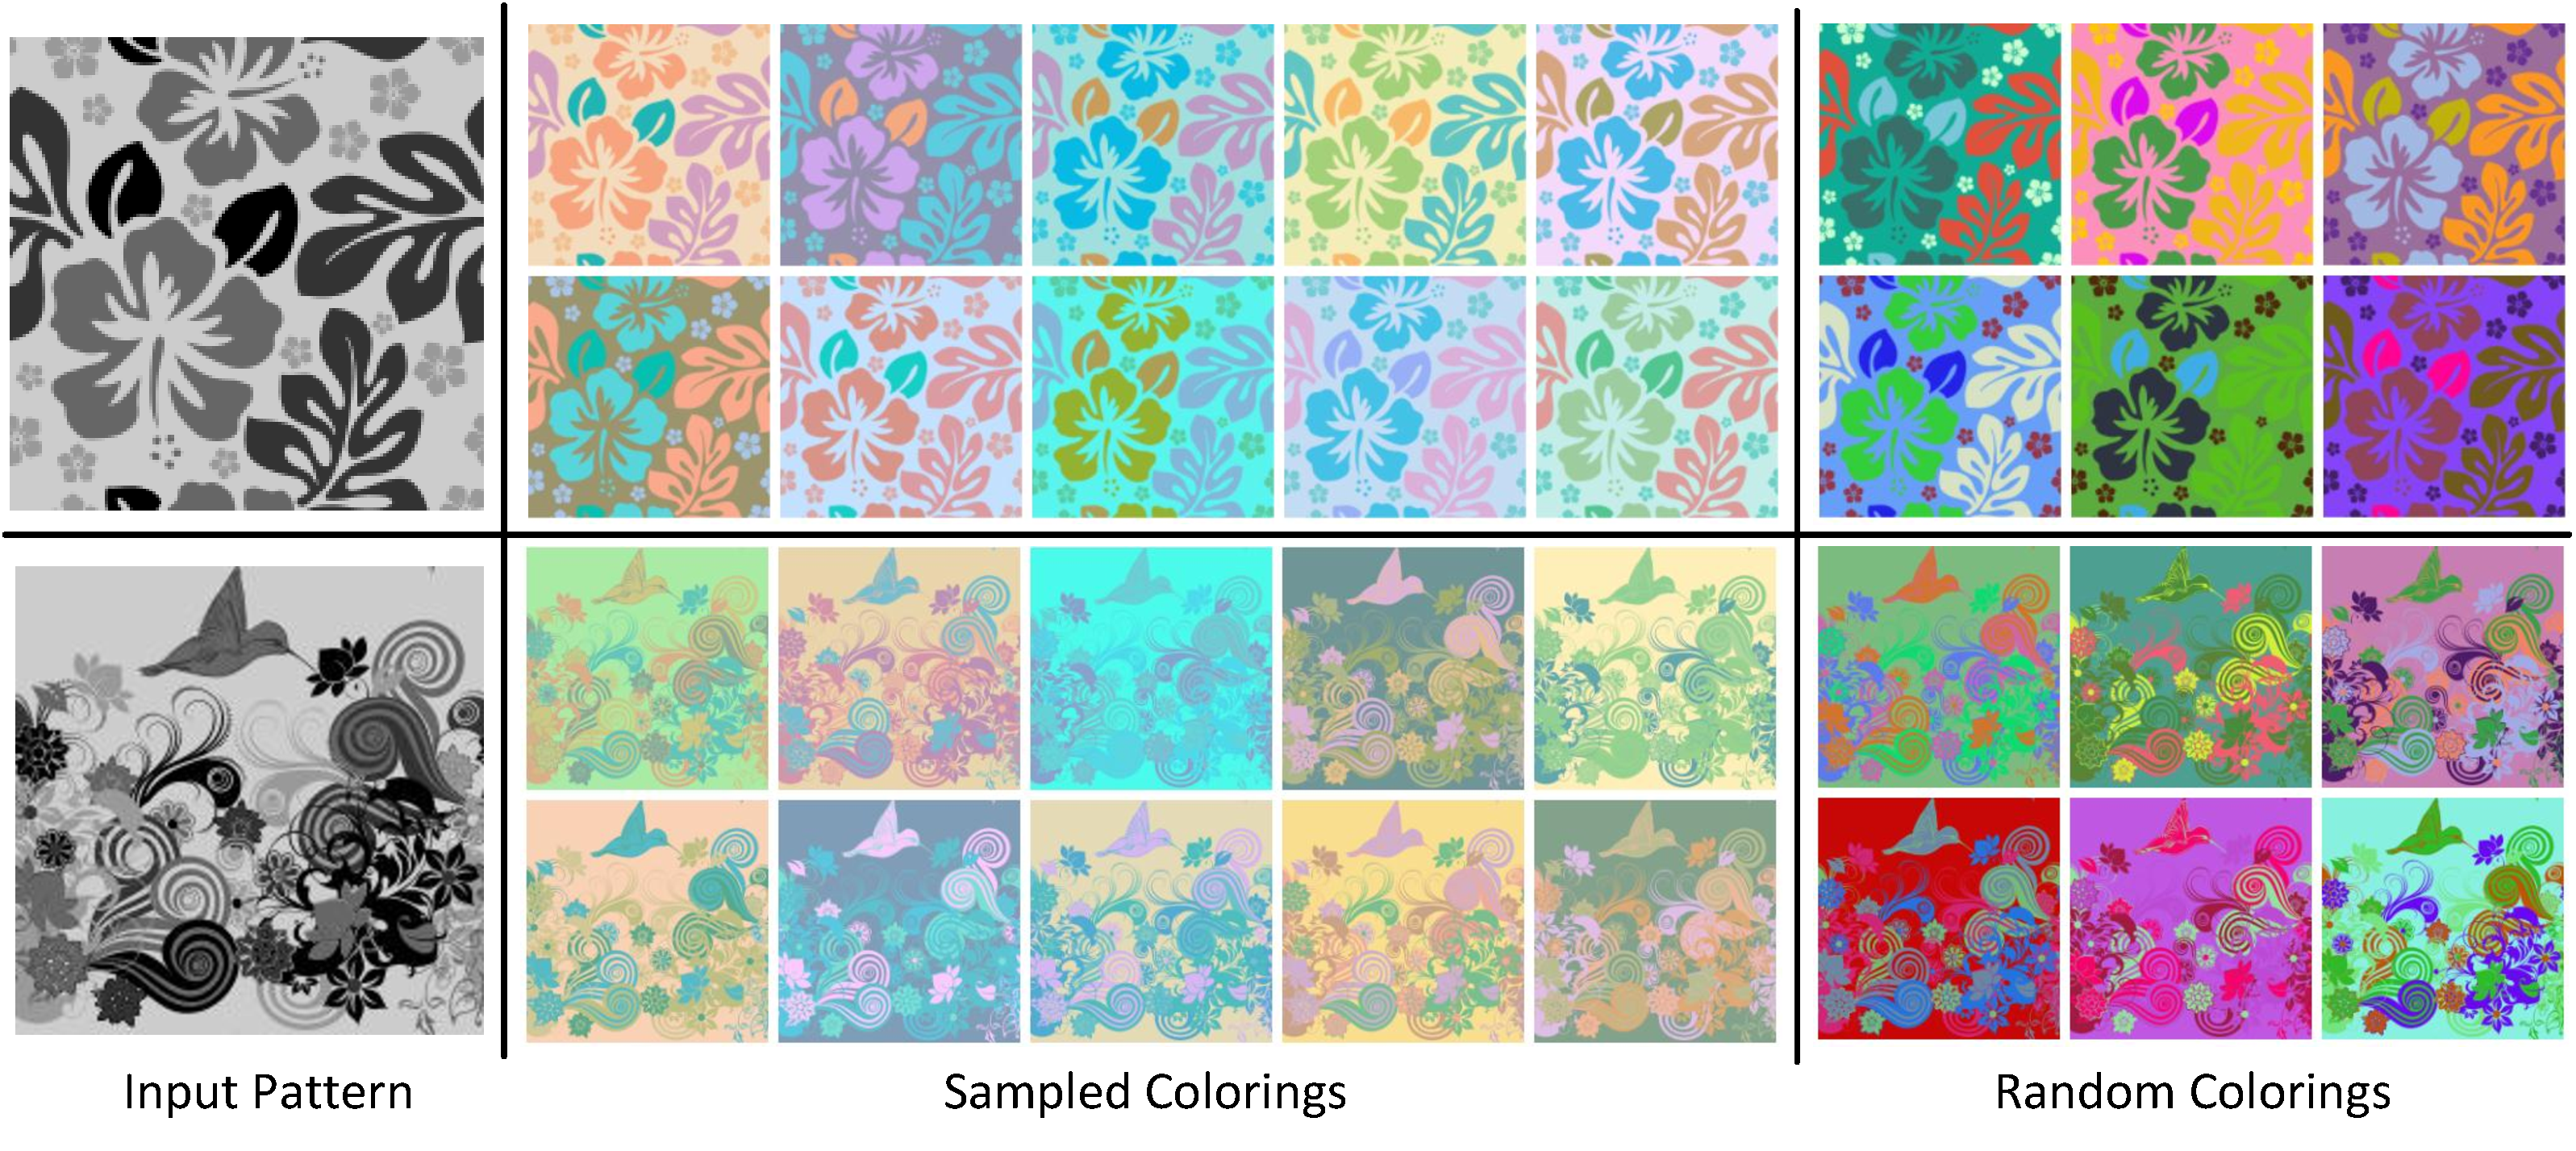
\includegraphics[width=\linewidth]{figs/teaser}
\caption{This is the awesome caption for the teaser!}
\label{fig:teaser}
\vspace{-1.0em}

}

\maketitle

\begin{abstract}
We present a method for automatically coloring 2D patterns. Our method uses a probabilistic factor graph model that can be sampled to generate new coloring suggestions. The model is trained on input example patterns to statistically capture the desirable stylistic properties of the inputs. Using Markov Chain Monte Carlo, the model can be sampled to generate a diverse set of attractive new colorings for a target pattern. This probabilistic framework is very general and allows for users to guide the generated suggestions via conditional inference or additional soft constraints. We demonstrate results on a variety of coloring tasks, and we evaluate the model through a perceptual study in which participants judged automatic colorings to be as desirable as hand-created ones.
\end{abstract}

%%% ACM Computing Review (CR) categories.
%%% See <http://www.acm.org/class/1998/> for details.
%%% The ``\CRcat'' command takes four arguments.

%\begin{CRcatlist}
%  \CRcat{I.3.5}{Computing Methodologies}{Computer Graphics}{Computational Geometry and Object Modeling};
%\end{CRcatlist}

\keywordlist
\copyrightspace

\TOGlinkslist

\section{Introduction}
\label{sec:introduction}

%% Hook and motivation
From graphic and web design, to fashion and fabrics, to interior design, colored patterns are everywhere. While almost anyone with normal color vision can distinguish patterns that they like from those they don't, \emph{creating} attractive patterns is difficult: it requires an extensive working knowledge of color and spatial aesthetics. For the purposes of this paper, we define a colored pattern to have two parts: a \emph{pattern template}, which specifies a creative decomposition of space into regions, as well as which regions must map to the same color; and a set of \emph{colors} assigned to those regions. Even the more constrained task of coloring an existing pattern template can be challenging, as it still exhbis a daunting array of coloring options. Experienced artists and enthusiasts often seek feedback and inspiration from online communities such as Colourlovers\footnote{http://www.colourlovers.com/}.

%% Goals
Can computation make the pattern coloring process easier for artists of all levels by automatically suggesting colorings? If a computational colorization tool existed, what criteria should it meet? Such a tool should be able generate pattern colorings that evoke a particular desired style, to accomodate different user preferences. It should generate a variety of different suggestions, so that an uncertain or inexperienced user can explore the space of possibilities. It should be able to generate suggestions automatically, but it should also expose controls for users to refine their criteria.

%% Challenges
Building such a system is difficult, as it requires a computational encoding of the properties that make a coloring desirable. There are many principles of aesthetics that might be relevant, such as any of the myriad of different color harmony rules~\cite{ColorHarmonyBook} or principles of art such as contrast and dominance~\cite{ArtPrinciples}. But which of these principles apply to which patterns? For those that do apply, which are the most important? Even assuming an answer to these questions, there is still the problem of how to actually \emph{generate} many, diverse new colorings that satisfy the desired properties.

%% Our approach
In this paper, we present a probabilistic approach to automatic pattern colorization. Our main contribution is a probabilistic factor graph model that can be trained on example patterns and sampled to generate new colorings for a target pattern template. The general-purpose factor graph framework allows us to incorporate terms in our model both for color compatibility and spatial consistency. The individual terms, as well as the relative importance of each term, are automatically trained using machine learning techniques, statistically capturing the desirable properties of the example patterns. By combining Markov Chain Monte Carlo sampling with sample-diversification techniques commonly used for information retrieval, our model can generate a wide variety of attractive colorings. And, via the use of conditional probabilistic inference or the addition of simple constraint factors, users can exercise a high degree of control over the generated suggestions.

%% Summary of results
We demonstrate the effectiveness of our model for a variety of constrained and unconstrained coloring suggestion tasks. We also show real-world applications of our automatic coloring system to 3D scene design and web design. Finally, we evaluate the quality of colorings generated by our model through a judgment study with people recruited online. Automatically-colored patterns were significantly preferred to random colorings and comparable to colorings made by an artist.
\section{Background}
\label{sec:background}

Related work has tackled problems similar to the one we address in this paper. While our approach builds on some of the ideas and algorithms presented in past research, these methods alone are not sufficient to meet the goals of this paper.

%\paragraph{Segmented image colorization}
\paragraph{Creative color support tools}
In the work most similar in goal to our own, Sauvaget and colleagues describe a system that takes as input an image divided into segments and a set of colors and computes a `harmonious' assignment of colors to segments, based on contrast of proportions guidelines ~\shortcite{ColorizationUsingHarmony}. The system selects colors from a fixed palette, and users can specify the set of colors to be used and their relative amounts in advance. However, these requirements can conflict with our goal of supporting exploratory coloring, in which the user may not know in advance the colors she wants, and would like to see many plausible suggestions. In contrast, our model is trained from artist-created images. It does not require the user to specify colors in advance, but its probabilistic inference framework is general enough to support this input if the user desires it.

In the theme of user exploration, Meier et al. develop a suite of interactive interfaces with a focus on helping users browse color themes and experiment with compositions~\shortcite{ColorPaletteTools}. However, they do not explore algorithms for generating coloring suggestions. In this paper, we explore generating algorithmic coloring suggestions while taking into account user input.

\paragraph{Color harmony \& compatibility}
%The computer graphics, aesthetics, and psychology literatures are replete with theories and models that try to capture the characteristics that make two or more colors compatible with one another~\cite{CohenOrHarmonization,Munsell,PalmerColorPreference}.
Computer graphics, aesthetics, and psychology literatures introduce many potential theories and models to explain and predict the compatibility of two or more colors~\cite{CohenOrHarmonization,Munsell,PalmerColorPreference}. Recently, O'Donovan and colleagues presented a data-driven model that predicts the numeric ratings people would give to five-color `color themes'~\shortcite{ODonovan}. This model is highly generalizable, and they demonstrate a variety of applications for it, including improving existing themes and suggesting colors to complete a partial theme. Our model includes this compatibility model as one of its terms. However, as we demonstrate in Section~\ref{sec:approach}, this term alone is insufficient to produce good colorings, as it does not take into account the spatial role each color plays in the pattern. Thus, our model uses the distinguishing features of each pattern region and the relationships between regions to constrain the space of colorings that it will suggest.

\paragraph{Natural image colorization}
While there is little work directly addressing pattern colorization, researchers have developed many approaches to colorizing grayscale photographic images. Many of these methods rely either on direct color input from the user~\cite{ScribbleColorization} or from a `source image' whose color properties should be matched~\cite{TransferColorization}. However, there is one approach that works more automatically by using a set of example images as training data~\cite{MultimodalColorization}. This approach builds up multimodal distributions of color variability given local texture descriptors and combines these into a conditional random field with unary and binary energy terms. The minimum-energy configuration is then found using a graph cut algorithm. Our model employs similar local color distributions but bases them on features from variable-sized pattern regions, rather than small texture patches. We also cast the task of finding good colorizations as a probabilistic inference problem, rather than an optimization. This framework allows our algorithm to explore the space of colorings and suggest multiple good alternatives, whereas a graph cut approach will yield only a single global optimum.

\paragraph{3D model colorization}
Other recent work has tackled automatic coloring of 3D objects. The DressUp! system suggests plausible outfits---including colors for each clothing item---for virtual characters~\cite{DressUp}. It also employs the color compatibility function of O'Donovan et al.~\shortcite{ODonovan} as part of a probabilistic model, but it does not consider the spatiality of color beyond a top-to-bottom ordering. The Material Memex system models the context-dependent correlation between geometric shape and material properties of 3D object parts~\cite{MaterialMemex}. In a related fashion, the system presented in this paper models the context-dependent correlation between pattern regions and color properties of those regions. The Material Memex does not include any explicit consideration of color compatibility. Additionally, its use of multinomial factors requires a quantization of material configuration space. Since the Memex does not consider colors separately from materials, this quantization can greatly restrict the set of colors the model can possibly suggest. In contrast, our model uses continuous probability distributions.
\section{Approach}
\label{sec:approach}

\remark{D: Tom Funkhouser sold me on the value of this section, and one of the best examples from his papers is in http://www.cs.princeton.edu/~funk/pvg01.pdf. I actually like combining the Approach and Overview sections into one shorter section, though.}

Restate problem statement, why it's hard, and our approach (emphasizing the key idea)~\remark{Why it's hard: This might be the best place to show the results when we only use color compatibility, i.e. ``As a first approach, you might try using existing color compatibility models...'' and then show how that doesn't work, thus motivating the machinery we're about to describe.}

%Start of notes on pattern template terminology/definition.
Pattern Template terminology/definition
\remark{S: Do we want to use 'pattern template' or something more general like 'coloring template'?}
\remark{D: I'm fine with `pattern,' but `template' might be overloaded with `factor template,' if we need to use that term when describing the model.}
Our approach takes as input a pattern template and any user-provided guidelines if available, and outputs suggested colorings for that pattern template. A pattern template specifies which regions in an image can be colored in, and which regions must map to the same color. For example, an image of a flower on a background may have a template that specifies all petals of the flower must be the same color, and all background regions must be the same color. In the rest of the paper, we refer to the set of regions that map to the same color as a \emph{color group}. Figure~\ref{fig:teaser} shows an example of a pattern template visualized in grayscale, where each different lightness level identifies a different color group. This pattern template representation is relatively easy to author from images composed of segments, such as website design, renderings of 3D scenes, and line drawings. In this paper, we focus on 2D graphic design patterns. 
%S: An alternative description of a pattern template: A pattern template is a segmented image with additional specifications on which segments must have the same color, or in other words, belong to the same color group

%TODO: Mention/Describe Colourlovers dataset somewhere. Briefly describe image preprocessing, and final renderings (probably this will be in the probabilistic model section?). 


%The (log linear) factor graph formalism (and any other persistent terminology).
\remark{S: An initial attempt at notation. Not sure if the general log-linear form equations are needed, since we'll go into specifics later and it might be confusing.}

We model the pattern colorization problem as a factor graph where the variables are the color groups $G_i$ and values are colors. We parameterize the likelihood of a color assignment as $P(G_1,..,G_n) \propto \prod_{i=1}^{k} \phi(D_i)$ where $D_i$ is some subset of variables. The factors $\Phi$ have the general log-linear form $\Phi(D_i) = exp(\sum_{j=1}^{m_i} \theta_j f_j(D_i))$ where $f_j(D_i)$ is some scoring function over $D_i$ and $\theta_j$ are weights. The log-linear form compactly represents the distribution of color assignments where the variable domain is potentially the whole color space. In addition, we can take advantage of well-established sampling techniques such as Markov-Chain Monte Carlo (MCMC) to generate multiple alternative colorings.


% Examples of similar cases where factor graphs have been used (does image segmentation/labeling count?)

Roadmap for the next section (which describes the technical details) / overview of the system.
\section{Probabilistic Model}
\label{sec:model}

We have defined unary, pairwise, and global scoring functions for pattern color properties. Now, we combine them into one scoring function that evaluates the overall quality of a pattern coloring.

For this task, we turn to the language of \emph{probabilistic factor graphs}. A factor graph is a probabilistic graphical model that decomposes a complex probability distribution over multiple variables into a set of smaller \emph{factors} over subsets of the variables. In our case, the variables $\colorVars$ are the colors of each color group in a pattern, and the factors $\factor$ are derived from our scoring functions. Figure~\ref{fig:FactorGraph} shows an example of a factor graph for one simple pattern. The circles denote color variables, while squares denote different factors $\factor$. Edges in the graph connect each factor to the variables within its scope.

\begin{figure}[ht]
%\raisebox{4em}{
\includegraphics[width=.2\columnwidth]{figs/factorGraphPattern}} &
%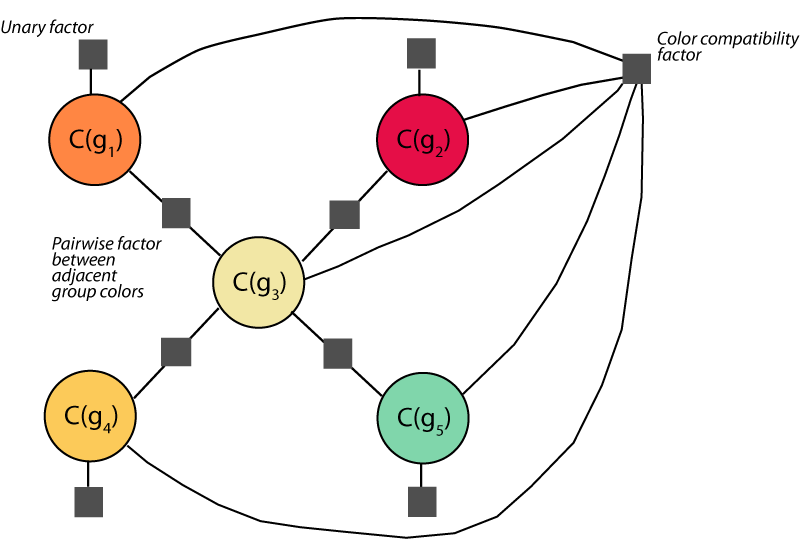
\includegraphics[width=.7\columnwidth]{figs/factorGraph} 
\centering
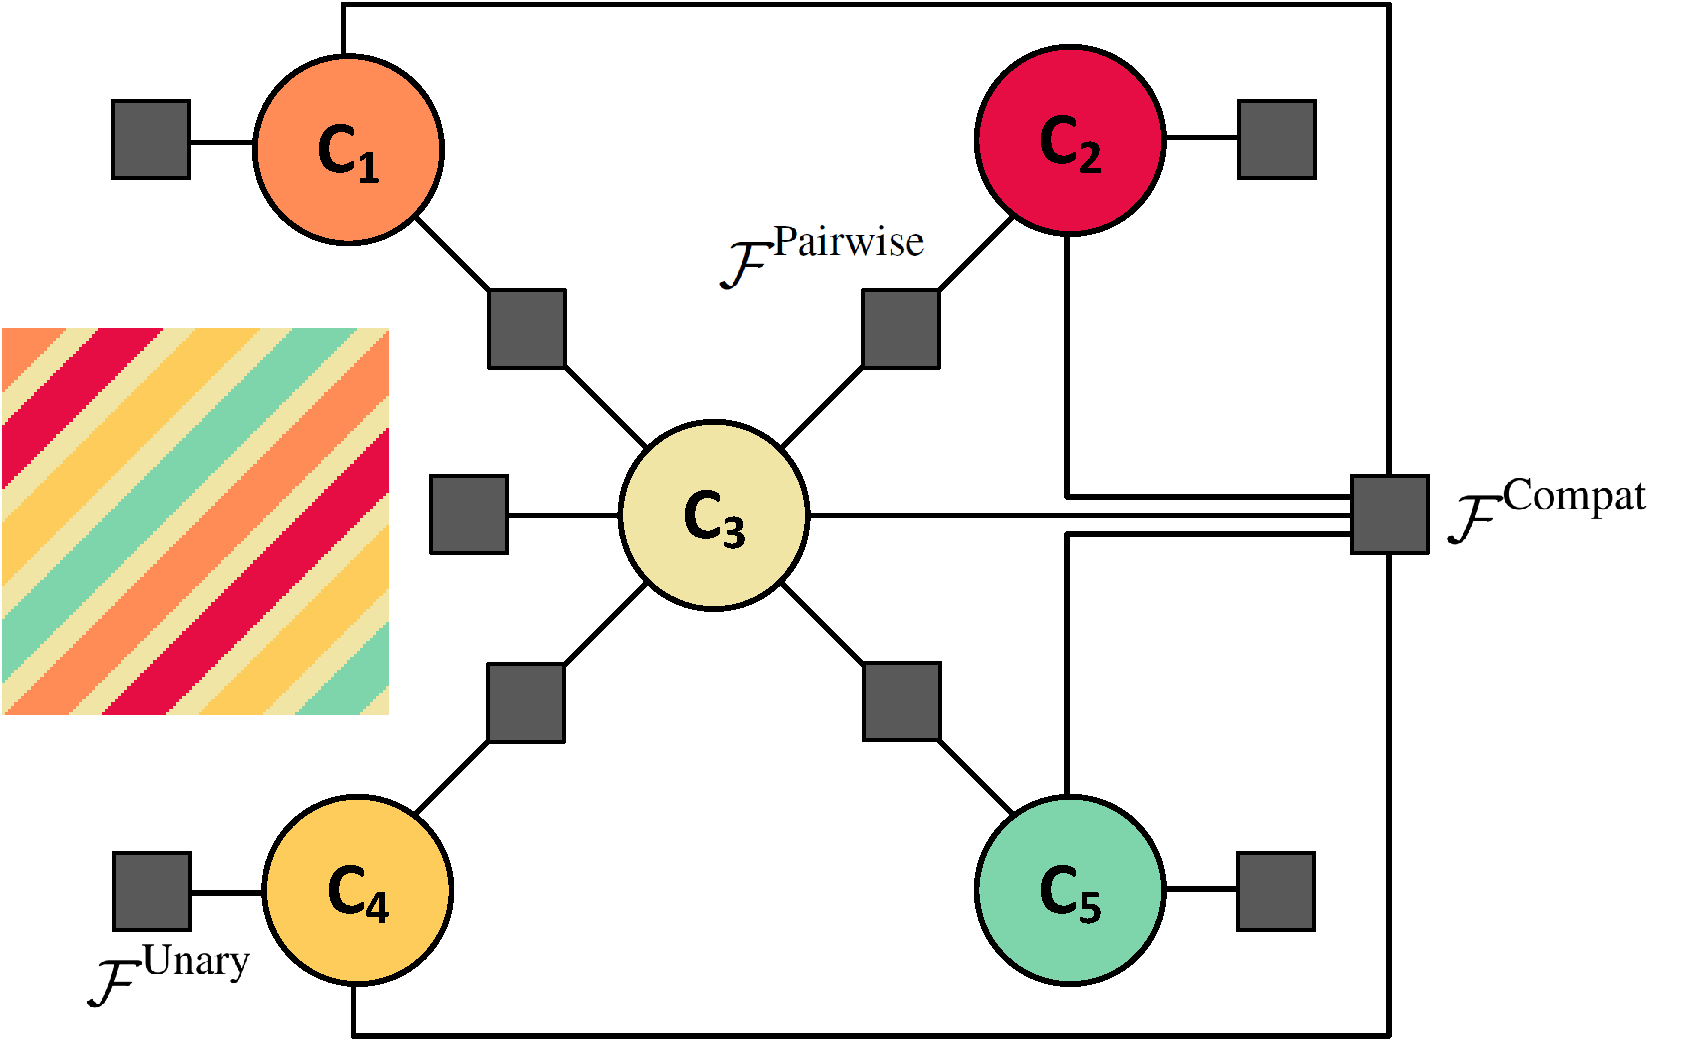
\includegraphics[width=0.85\columnwidth]{figs/factorGraphNew}
\caption{A factor graph for an example pattern template. Variable nodes are colored according to their corresponding color group in the pattern.}
\label{fig:FactorGraph}
\end{figure}

The factors connected to a single variable are derived from our unary scoring functions; they combine the score for a color group with the scores for all segments in that group:
%%
\begin{equation*}
 \factor^{\textrm{Unary}}_\prop(\colors_\group) =
 		\exp( \groupTermWeight \cdot \groupInstStats(\colors_\group)  \\
 		     + \segTermWeight \cdot \sum_{\segment \in \group} \segInstStats(\colors_\group)) 
\end{equation*}
%%
The $w$'s are weights that control the relative importance of each function; we will see how to set them later in this section.

The factors connecting two variables come from our pairwise scoring functions and combine the scores for all adjacencies which involve segments from two different color groups:
\begin{equation*}
\factor^{\textrm{Pairwise}}_\prop(\colors_\group, \colors_\groupprime) =
	\exp( \adjTermWeight \cdot \sum_{\mathclap{(\segment, \segprime) \in \adj(\group, \groupprime)}} \adjInstStats( \colors_\group, \colors_\groupprime))
\end{equation*}
%%
Finally, the factor connected to all five color variables enforces color compatibility:
%%
\begin{equation*}
\factor^{\textrm{Compat}}(\colors_1 \ldots \colors_5) = \exp(\colorCompatWeight \cdot \colorCompatInstStats(\colors_1 \ldots \colors_5))
\end{equation*}
%%
The probability distribution encoded by this factor graph is the normalized product of all of these factors:
%%
\begin{equation*}
p(\colors | \pattern : \weights) = \frac{1}{Z(\pattern : \weights)} \prod_{\factor} \factor(\textit{Scope}_\factor(\colors))
\end{equation*}
%%
Here, $\textit{Scope}_\factor$ selects the color variables connected to the factor $\factor$ and $Z(\pattern : \weights)$ is the pattern-dependent partition function that normalizes the distribution. The distribution is parameterized by the vector of factor weights $\weights$.


\subsection{Sampling}
\label{sec:sampling}

Generating good coloring suggestions reduces to sampling high-probability colorings from our model. We use the Metropolis-Hastings algorithm (MH), a variant of Markov Chain Monte Carlo (MCMC)~\cite{Metropolis,Hastings}. MH explores the coloring state space by \emph{proposing} candidate new states, which are accepted with probability proportional to their model score. We would also like our sampler to output a variety of suggestions, which requires that it explore many modes of the distribution. To do this efficiently, we use parallel tempering, a technique that runs multiple MCMC chains in parallel at different `temperatures' and swaps their states periodically~\cite{ParallelTempering}. `Hot' chains are more likely to take large jumps across the state space, whereas `cool' chains behave like local hill-climbing optimizers. The combined system of chains effectively explores and refines different coloring configurations.

Our sampler uses the following MH proposals:
\begin{itemize}
	\item{\textbf{Perturb} a randomly chosen color by $v \sim \mathcal{N}(0, \sigma)$ in RGB space}
	\item{\textbf{Swap} two randomly chosen colors}
\end{itemize}
where $\sigma$ varies linearly with the model temperature $t$, encouraging larger perturbations at high temperatures. The sampler chooses between these two proposals with a probability that also varies linearly with temperature. The sampler operates in RGB space since all RGB colors fall in the display gamut---which is not the case with \lab space---and the sampler should not waste time exploring colorings that cannot be visualized. Since the RGB color space is bounded, the perturbation proposal draws from a truncated normal distribution in order to maintain ergodicity of the MCMC chains~\cite{TruncatedGaussians}.

Finally, we use maximimum marginal relevance (MMR) to enforce diversity in the set of suggestions returned by the sampler~\cite{MMR}. MMR is a technique from information retrieval that re-ranks every item in a list according to a linear combination of relevance (model score, in our case) and similarity to the items preceding it. The similarity metric we use for two colorings $\colors$ and $\tilde{\colors}$ of a pattern is $- \sum_{\group \in \groups} {\size_\group \cdot ||\colors_\group - \tilde{\colors}_\group||}$, which is the area-weighted sum of \lab distances between the corresponding colors in each coloring.

\subsection{Weight Learning}
\label{sec:weights}

The factor graph model we have defined is parameterized by a vector of weights $\weights$. Setting these weights manually proves challenging, as it is not obvious which color properties matter most to the quality of a pattern coloring. Instead, we would like to set them automatically, using our training dataset as a guide.

We formulate the weight-tuning problem as one of \emph{maximum likelihood parameter estimation}: we would like to set the weights such that the training examples have high probability under the resulting model. We first rewrite the probability distribution encoded by our model from a weight-centric view
%%
\begin{equation*}
p(\colors | \pattern : \weights) = \frac{1}{Z(\pattern : \weights)} \prod_{w \in \weights} \exp(w \cdot \weightStats(\colors, \pattern))
\end{equation*}
%%
where $\weightStats(\colors, \pattern)$ sums all the scoring functions $\phi$ that share the weight $w$. We can then express the log-likelihood of the weights given a dataset $\dataset$ of pattern colorings:
%%
\begin{equation*}
\ell(\weights : \dataset) =
	\sum_{(\pattern, \colors) \in \dataset}
	(
		\sum_{w \in \weights}
			w \cdot \weightStats(\colors, \pattern)
	)			
		- \ln{Z(\pattern : \weights)}
\end{equation*}
%%
Convex log-likelihoods such as this are typically maximized via gradient ascent. The partial derivatives of this function with respect to the weights are
%% Partial derivatives
\begin{equation*}
\frac{\partial}{\partial w} \ell(\weights : \dataset) = 
	\sum_{(\pattern, \colors) \in \dataset}
			\weightStats(\colors, \pattern)
		- \expectation_\weights[\weightStats(\colorVars, \pattern)]
\end{equation*}
%%
where $\expectation_\weights$ denotes an expectation under the model with weights $\weights$. Unfortunately, these quantities are extremely expensive to compute: the expectation term requires probabilistic inference---an NP-complete problem---for every training pattern, for every iteration of gradient ascent.

This computational intractability has motivated the development of alternative, `biased' parameter estimation schemes which do not directly maximize the likelihood function but nevertheless yield parameters that give high likelihoods. We use one such method called \emph{Contrastive Divergence} (CD)~\cite{ContrastiveDivergence}. CD uses the following approximation to the likelihood gradient:
%% CD gradient
\begin{equation*}
CD^k_w(\weights : \dataset) = 
	\sum_{(\pattern, \colors) \in \dataset}
			\weightStats(\colors, \pattern)
		 -\weightStats(\hat{\colors}, \pattern)
\end{equation*}
%%
where $\hat{\colors}$ is the coloring obtained by running an MCMC chain for $k$ steps from the initial coloring $\colors$. CD forms a local approximation to the likelihood gradient around the neighborhood of $\colors$. Larger $k$ yields more accurate approximations at additional cost; we use $k = 10$. We initialize the weights uniformly to 1 and constrain them to be non-negative, since all terms in the model are log-probabilities.

While the exact weights learned depend on the training dataset, we have noticed several persistent trends.
The perceptual difference, color compatibility, and color name count terms receive the highest weights. These trends coincide well with our intuition that colors should be harmonious, adjacent regions should have sufficient contrast, and colors should be categorically similar to those in the training set.
The lowest weight belongs to the color name similarity term, which suggests that the similarity in how two colors are named is not strongly predictive of their compatibility as an adjacent color pair.
%The information conveyed by this property may be partially redundant with the perceptual difference term. Also, as this property computes the cosine similarity between two 179-dimensional color name count vectors, the dimensionality of the color name space may simply be too high to provide sufficient discrimination for pattern coloring.

\subsection{Implementation}
\label{sec:implementation}

Our prototype implementation of this model is written in the Scala programming language, using the Factorie toolkit for probabilistic modeling~\cite{Factorie}. To evaluate the color compatibility term, it uses the reference MATLAB implementation provided by O'Donovan et al.~\shortcite{ODonovan}.
%A link to the source code can be found on the project website.
\section{Results}
\label{sec:results}

The data-driven probabilistic model we have presented produces good-looking patterns and can be applied in many different ways. The factor graph representation makes it easy to adapt our framework to handle new problems or incorporate user-provided design constraints by introducing additional factors to the factor graph, or changing the source data used to train the factor weights and histograms.

\remark{Discuss parameters used to train model ``unless otherwise specified''. Number of artists, weights, etc. Say that the supplemental materials lists the patterns used in this training set.}
\remark{Because many patterns are recolorings of the same template, we make sure to separate our training and test sets so they do not share any templates}

The results shown below are rendered using the COLOURlovers interface, using color assignments generated by our model. 
%The results shown below are rendered from the original vector pattern using the Colourlovers interface, from color assignments generated by our model. 

\subsection{Coloring Pattern Templates}

\paragraph{Automatic pattern coloring} In the most direct application of our framework, we can sample from our model to produce colorings for a pattern template that are similar to the colorings used for training. Figure~\ref{fig:teaser} shows two examples of this process. The sampled patterns exhibit a range of colors and styles employed by the Colourlover artists. For comparison, the same patterns colored with palettes randomly sampled from RGB-space are shown on the right. These patterns exhibit significant problems, such as low color harmony and adjacent regions with equi-limuinant colors.

\begin{figure*}[ht!]
\begin{tabular}{ccc}

\includegraphics[width=.15\linewidth]{figs/permutationTemplatePalette} & 
\includegraphics[width=.4\linewidth]{figs/permutationBest8} & 
\includegraphics[width=.4\linewidth]{figs/permutationWorst8} %& 
\includegraphics[width=.12\linewidth]{figs/permutationArtist}
  \\
\textbf{(a)} Input Pattern & \textbf{(b)} Highest-scoring assignments & \textbf{(c)} Lowest-scoring assignments %& \textbf{(d)} Artist assignment
\\
\end{tabular}

\caption{Given a segmented image and corresponding palette as input, we use our color model to compute the likelihood of each possible assignment of the palette to the image regions. \textbf{(b)} and \textbf{(c)} show the top-eight and bottom-eight assignments. The assignment provided by the artist received the second-highest score and is highlighted in blue.}
\label{fig:permutation}
\end{figure*}


\begin{figure}[ht!]
\begin{tabular}{cccc} 
\raisebox{0.5em}{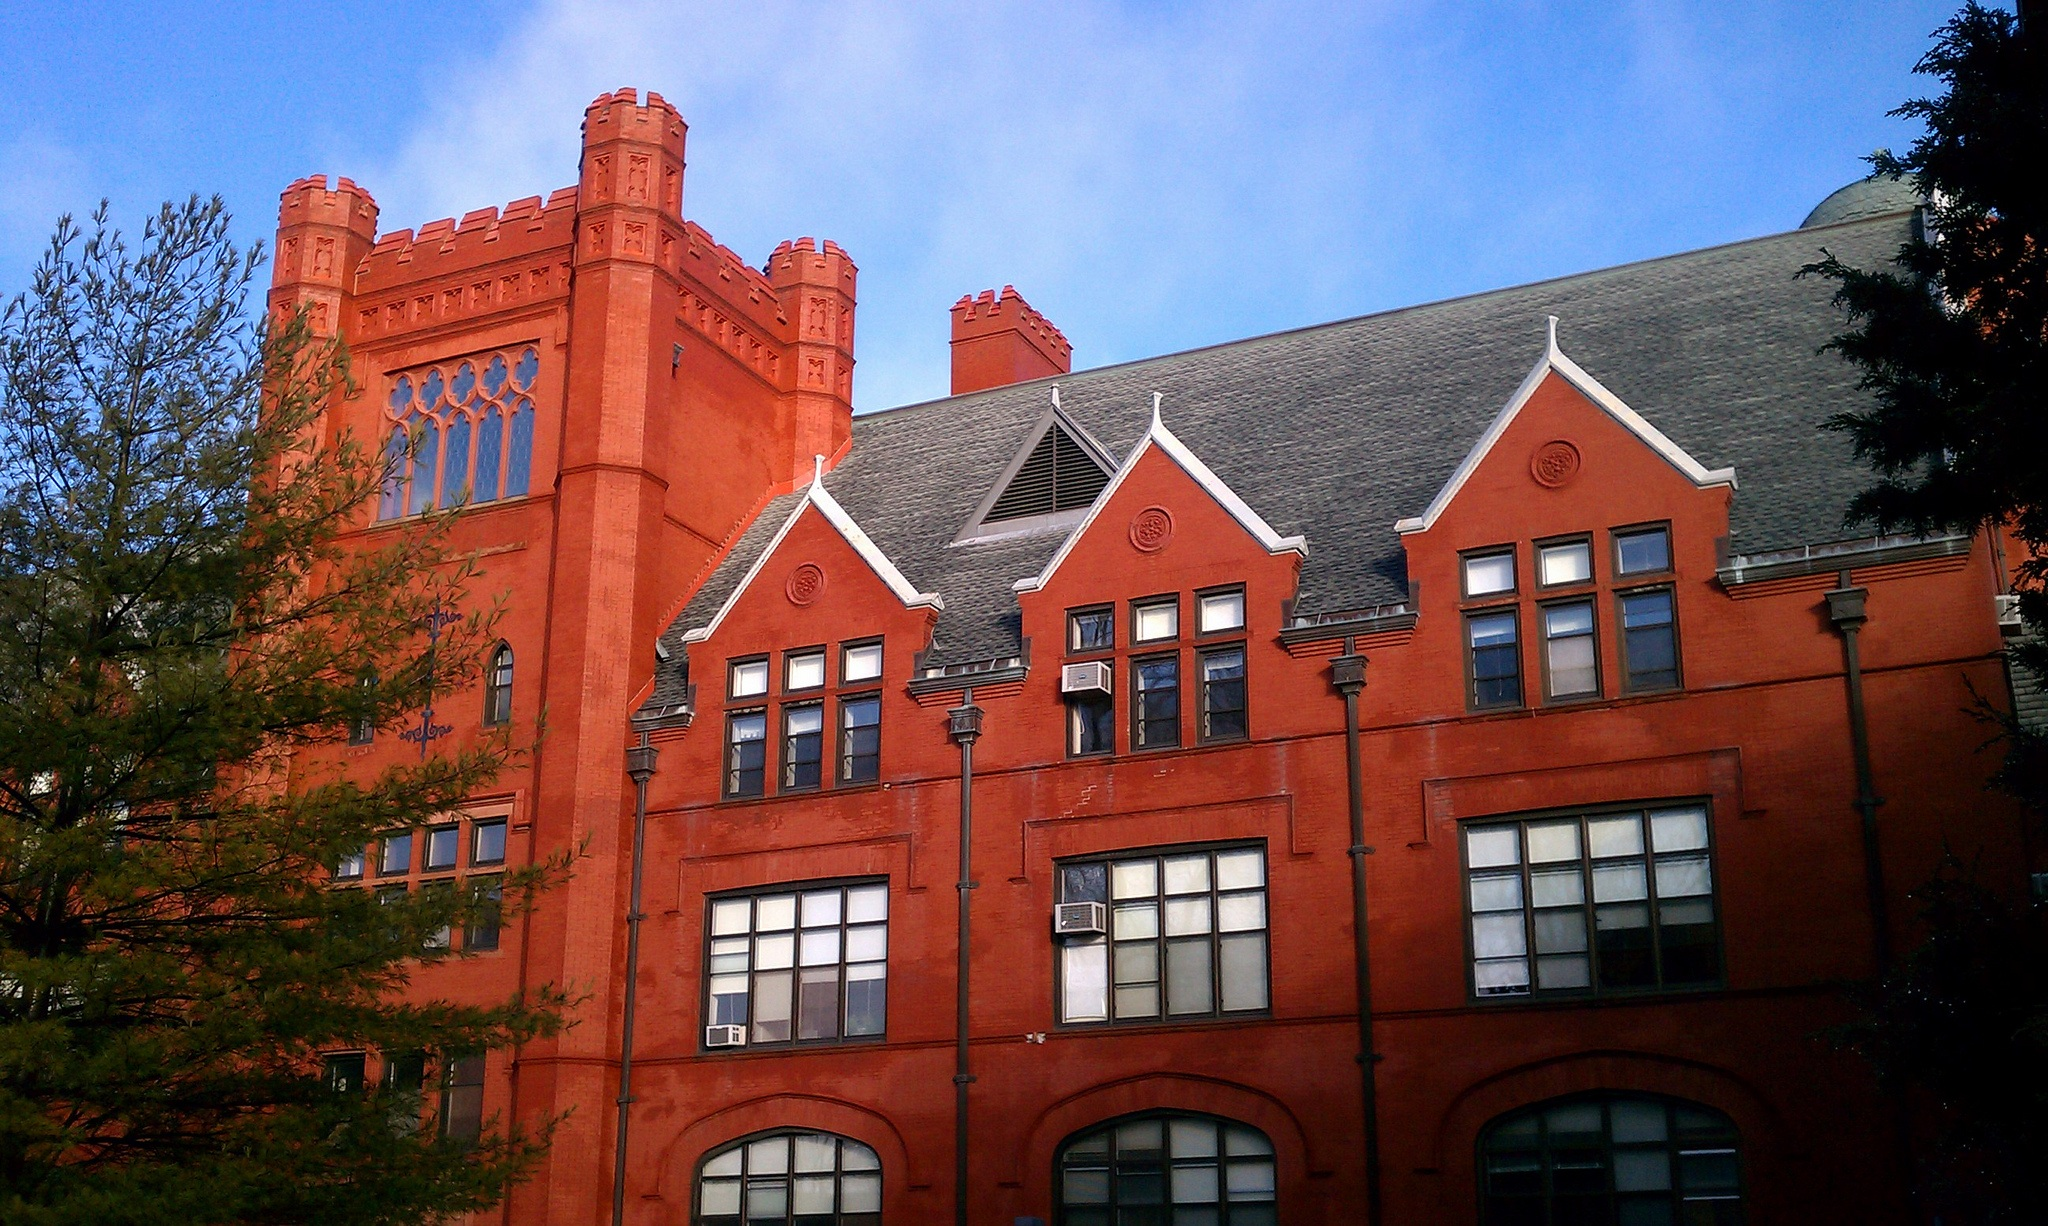
\includegraphics[width=.275\columnwidth]{figs/photos/brick}}&
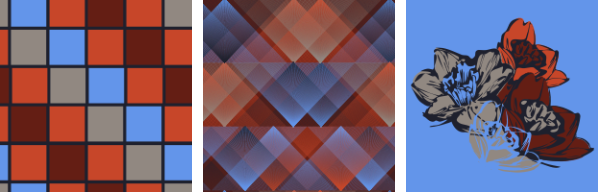
\includegraphics[width=.65\columnwidth]{figs/photos/brickAll}\\
\raisebox{0.5em}{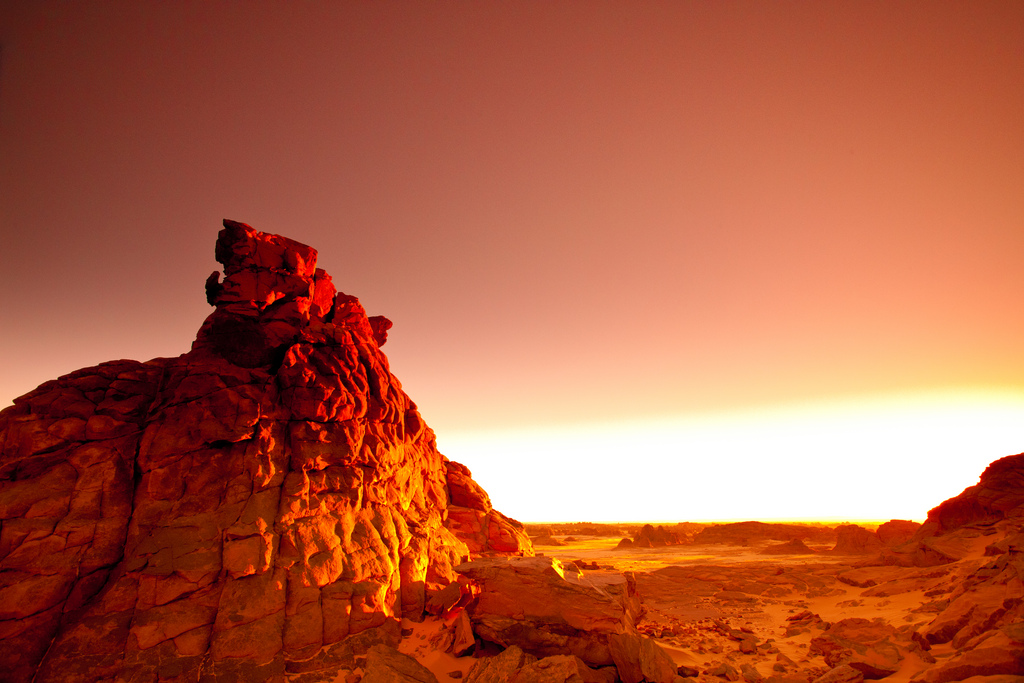
\includegraphics[width=.275\columnwidth]{figs/photos/sunset}}&

\includegraphics[width=.65\columnwidth]{figs/photos/sunsetAll}
\end{tabular}

\caption{Palettes are extracted from the two input photographs on the left, and on the right we show the top-scoring coloring suggested by our algorithm for three different pattern templates.}
\vspace{-1.0em}
\label{fig:photographMatching}
\end{figure}

\paragraph{Coloring with fixed palettes} In some cases, an artist already knows what colors she wants to use in an image. She might have found a palette she is enamored with elsewhere or may have a very specific theme in mind. Even with a fixed palette, there are still a range of images that can be created by mapping different colors to different regions, only some of which are desirable. To support this task, we use our model's score to rank all possible permutations of the colors. Figure~\ref{fig:permutation} shows one example of this process. \ref{fig:permutation}b shows the eight highest-rated color assignments which exhibit a variety of color styles, such as using four different background colors. On the other hand, the lowest-rated assignments all use the tangerine background color. Our color model assigns a very low score to using this color for the background region because its color properties are not similar to background colors in the training set. The actual color assignment originally provided by the artist for this color template received the second-highest score, suggesting that our model was able to capture the artist's intent. Figure~\ref{fig:photographMatching} shows another application, where the input palette is instead derived from an input photograph~\cite{SharonPaletteExtraction}. Our algorithm automatically computes a pleasing mapping from the colors in the extracted palette to regions in a given pattern template.

\paragraph{Hard color constraints}

\begin{figure*}[ht!]
\begin{tabular}{cc} 

\includegraphics[width=.475\linewidth]{figs/constrainedSearchUnconstrained}&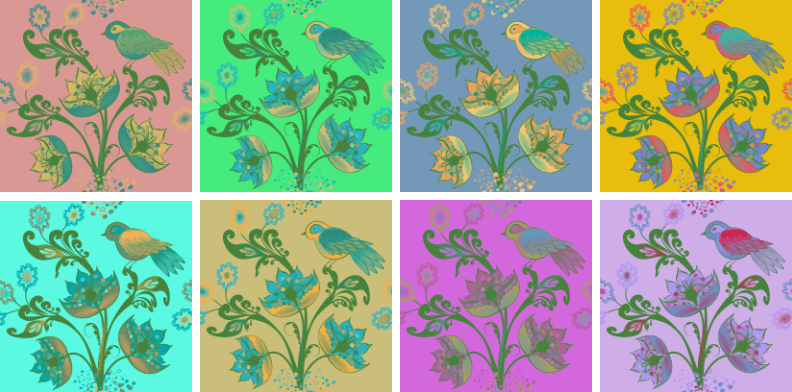
\includegraphics[width=.475\linewidth]{figs/constrainedSearchConstrained}\\
Unconstrained sampling&Constrained sampling\\
\end{tabular}

\caption{An artist coloring a pattern is presented with the results shown on the left, and decides that she only likes results where the stem of the plant is dark green. On the right, we use conditional inference to sample from our model subject to the constraint that the desired palette entry is fixed to a specific color. This is a natural way to incorporate semantic information about region colors which our model cannot capture.}
\label{fig:constrainedInference}
\vspace{-1.0em}
\end{figure*}

A user coloring a pattern may be confident about the colors he wants to see in some regions but uncertain about others. Our model can assist users in this situation by fixing the color of certain pattern regions and using conditional inference to sample values for the remaining unconstrained color variables. Figure~\ref{fig:constrainedInference} shows an example, in which the model samples from the highest-scoring patterns subject to the constraint that the plant stem must be a specific shade of green.

\paragraph{Soft color constraints}

In another use case, a user might manually color a pattern and then wish to see variations upon this theme, hoping to find better-looking alternatives nearby in the space of colorings. Our model can support this type of query by incorporating an additional soft constraint factor on color variable, constraining it ot be close to a target color:
%%
\begin{equation}
\factor^\textrm{Target}(\colorVars_\group | \pattern) = \mathcal{N}(||\colorVars_\group - \textrm{targetColor}(\group)||, \sigma_\textrm{user})
\label{eq:targetFactor}
\end{equation}
%%
Here, $\textrm{targetColor}(\group)$ is the desired color of group $\group$ and $\sigma_\textrm{user}$ controls the extent to which the group is allowed to deviate from the desired color. We assign this factor a weight $w_\textrm{user} * w_\textrm{model}$, where $w_\textrm{model}$ is the sum of the weights of all other factors in the model. $w_\textrm{user}$ controls the tradeoff between satisfying the user-specified target colors for a region versus satisfying the color distribution encoded by the trained model.
%
%This factor corresponds to adding a new term in our log-linear model with this statistics function:
%%%
%\begin{equation*}
%\termStats(\colors | \pattern) = \sum_{\group \in \groups}{\ln \mathcal{N}(||\colors_\group - \textrm{targetColor}(\group)||, \sigma_\textrm{user})}
%\end{equation*}
%%%

\begin{figure}[ht!]
\begin{tabular}{cc}
\raisebox{2em}{
\includegraphics[width=.22\columnwidth]{figs/guidedSearch1Original}}&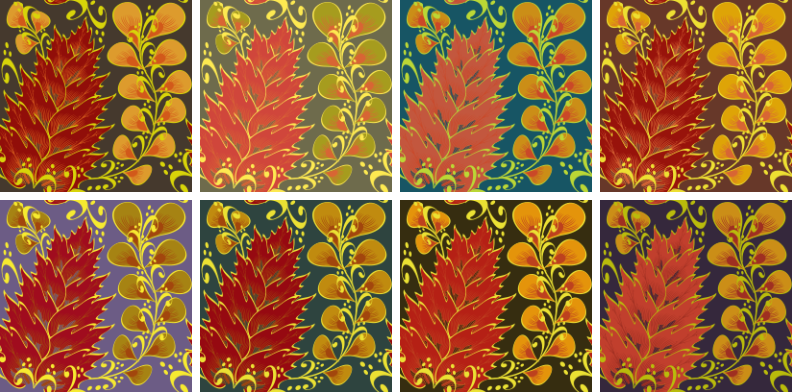
\includegraphics[width=.7\columnwidth]{figs/guidedSearch1MMR}\vspace{0.5em}\\
\raisebox{2em}{
\includegraphics[width=.22\columnwidth]{figs/guidedSearch0Original}}&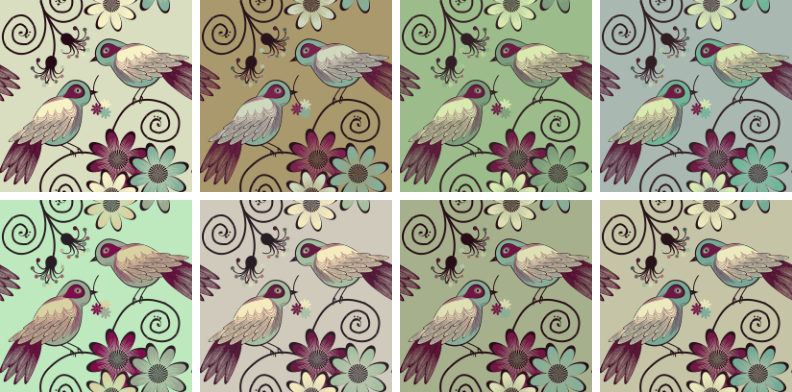
\includegraphics[width=.7\columnwidth]{figs/guidedSearch0MMR}\vspace{0.5em}\\
%\raisebox{2em}{
\includegraphics[width=.22\columnwidth]{figs/guidedSearch2Original}}%&
\includegraphics[width=.7\columnwidth]{figs/guidedSearch2MMR}\\
Suggestion&Results\\
\end{tabular}

\caption{An artist provides an initial color assignment and asks for patterns that are similar. We incorporate this request by adding an additional factor to our model, showing eight samples drawn from the new model for each of the suggested images.}
\label{fig:nearbySuggestions}
\vspace{-1.0em}
\end{figure}

Figure~\ref{fig:nearbySuggestions} shows example scenarios where a proposed coloring is given, and the model returns similar colorings.

\begin{figure}[ht!]
\begin{tabular}{ccc} 
Style&Example&Results\\ %\hline
\raisebox{1.55em}{\emph{Light}}&
\includegraphics[width=.148\columnwidth]{figs/styleResultsLightExample}&
\includegraphics[width=.62\columnwidth]{figs/styleResultsLight}\vspace{0.5em}\\
\raisebox{1.55em}{\emph{Dark}}&
\includegraphics[width=.148\columnwidth]{figs/styleResultsDarkExample}&
\includegraphics[width=.62\columnwidth]{figs/styleResultsDark}\vspace{0.5em}\\
\raisebox{1.55em}{\emph{Bold}}&
\includegraphics[width=.148\columnwidth]{figs/styleResultsBoldExample}&
\includegraphics[width=.62\columnwidth]{figs/styleResultsBold}\vspace{0.5em}\\
\raisebox{1.55em}{\emph{Mellow}}&
\includegraphics[width=.148\columnwidth]{figs/styleResultsMellowExample}&
\includegraphics[width=.62\columnwidth]{figs/styleResultsMellow}\vspace{0.5em}\\
\end{tabular}

\caption{In this example, 17 patterns were chosen in three different styles, and a representative image from each style is shown in the second column. A separate model was then trained on each style, and in the third column we show four samples drawn from each model. In each case, our model is able to learn different properties of the desired distribution over colors.}
\label{fig:styleTraining}
\vspace{-1.0em}
\end{figure}

\begin{figure*}[ht!]
\begin{tabular}{cc} 

\includegraphics[width=.48\linewidth]{figs/styleSugarExamples}&
\includegraphics[width=.48\linewidth]{figs/styleAlbenajExamples}\vspace{1.0em}\\

\includegraphics[width=.48\linewidth]{figs/styleSugar}&
\includegraphics[width=.48\linewidth]{figs/styleAlbenaj}\\
Artist A&Artist B\\
\end{tabular}

\caption{Our data-driven approach makes it easy to capture the styles of different artists. Top: representative images from two different artists. Bottom: results sampled from a model trained on 100 images from the artist.}
\vspace{-1.0em}
\label{fig:artistTraining}
\end{figure*}

\paragraph{Style capture} A powerful advantage of a data-driven approach is the ability to modify the underlying training source to achieve specialization of the resulting model. This ability allows our model to capture a specific style and color preferences such as ``high-contrast patterns'' simply by selecting a set of patterns with the desired property. Figure~\ref{fig:styleTraining} demonstrates this behavior using four style categories: \emph{Light}, \emph{Dark}, \emph{Bold}, and \emph{Mellow}. With only 17 training examples, our model can still capture general properties of the example patterns such as the distribution of colors over the background regions in \emph{Light} and \emph{Dark} and the amount of contrast between regions in \emph{Bold} and \emph{Mellow}. The model can also capture the style of a specific artist, as shown in Figure~\ref{fig:artistTraining}. Here, 100 images from each artist were used for training. The sampled images mimic certain properties of the the style of each artist, such as the light backgrounds preferred by artist A and the bold colors and dark backgrounds preferred by artist B. The complete list of patterns used as training data for these examples can be found in the supplemental materials.

\subsection{Applications}

\paragraph{Web design}
Our model can assist web designers by suggesting recolorings for web page pattern elements. In Figure~\ref{fig:webpageRecoloring}, the background pattern of a blog is recolored according to different seasons; the blog author could use a different coloring depending on the time of year. We generate these recolorings by adding new factors to the model. First, we add a unary factor to each color variable that encourages it to be similar to a color that occurs in the web page body:
%%
\begin{equation*}
\factor^\textrm{WebSim}(\colorVars_\group | \webpage) = p(\colorVars_\group | \webpage)
\end{equation*}
%%
where $\webpage$ is a rendered image of the web page body. The distribution $p$ is represented with a smoothed histogram of colors in the image, after quantizing to a small number of colors (20, in this experiment).
We also add a factor to the pattern's background color group (assumed to be the largest color group in the pattern) that penalizes it for being too similar to the web page body background color:
%%
\begin{equation*}
\factor^\textrm{BgPen}(\colorVars_{\textrm{largest}(\groups)} | \webpage) = 0.05 \cdot || \colorVars_{\textrm{largest}(\groups)} - \textrm{bgColor}(\webpage) ||
\end{equation*}
%%
Incoporating this term ensures that the body of the page stands out from the rest of the page. A more sophisticated approach would consider the entire web page to be a pattern and perform joint recoloring; we leave this extension to future work.


\begin{figure}[ht!]
\centering

\includegraphics[width=\columnwidth]{figs/webpageRecoloring}
\caption{With a few additional factors, our model can recolor the background of a web page in concert with the colors in the page body. (Top) A Spring-themed seasonal recoloring. (Middle) A Summer-themed recoloring. (Bottom) A Winter-themed recoloring. Design adapted from \url{www.thedesigncubicle.com}}
\label{fig:webpageRecoloring}
\end{figure}

\paragraph{3D scene design}
Color-coordinating a virtual scene is another creative task that can benefit from computatational support. While repositories such as the 3D Warehouse provide a wealth of object models with which to build scenes, and prior research has investigated computational support for arranging those objects~\cite{SceneSynth}, coloring them in a consistent and pleasing way remains challenging. Figure~\ref{fig:sceneRecoloring} shows how our model can make this task easier. In this example, the original scene is composed of models whose material colors are internally consistent but do not harmonize with each other; this is a common problem when constructing scenes from repository models. We can treat this scene as a recolorable pattern by rendering its material coefficients to an image. The user then provides a few additional annotations to specify which object components should take the same color; in this example, all cushions, pillows, and wooden objects must take the same color. Finally, we add a factor to our model to enforce that the colors assigned to each component are similar to their original colors (see Equation~\ref{eq:targetFactor}). The resulting model, when sampled, suggests plausible, improved recolorings of the scene. Our model's applicability to this task, despite it being trained only on \emph{2D} patterns, suggests that it captures some simple cross-domain aesthetic principles.

\begin{figure*}[ht!]
\begin{tabular}{c|ccc} 
Original&Recoloring 1&Recoloring 2&Recoloring 3\vspace{0.4em}\\
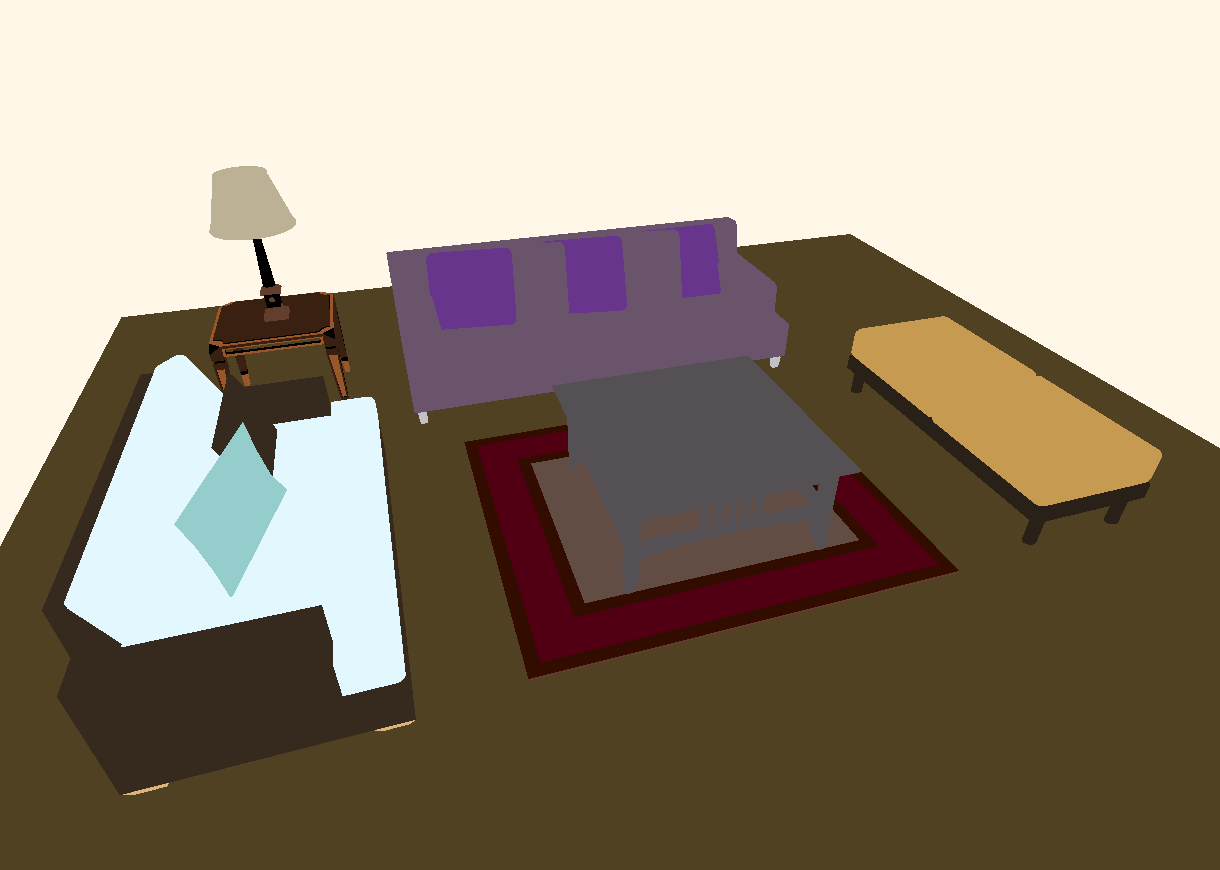
\includegraphics[width=.23\linewidth]{figs/3dscene/original}&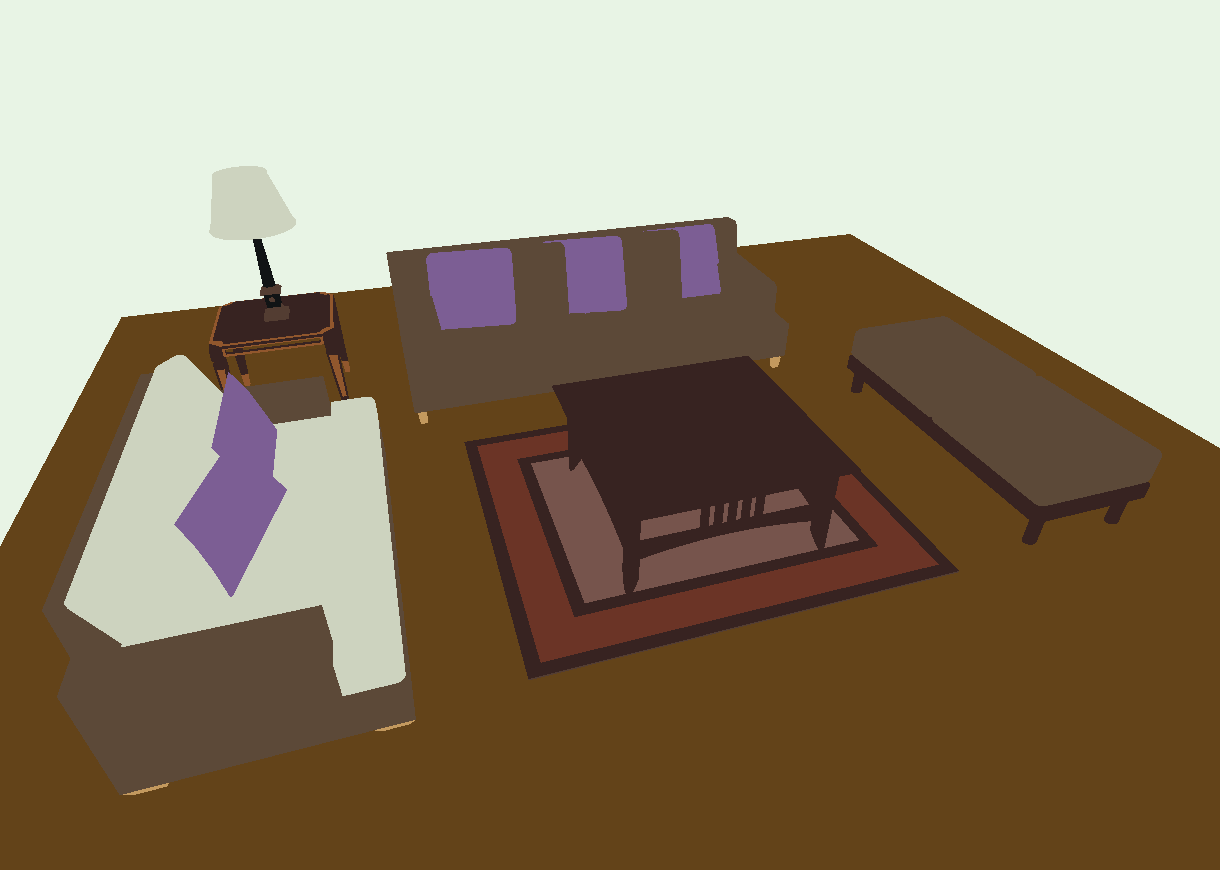
\includegraphics[width=.23\linewidth]{figs/3dscene/recolored_00}&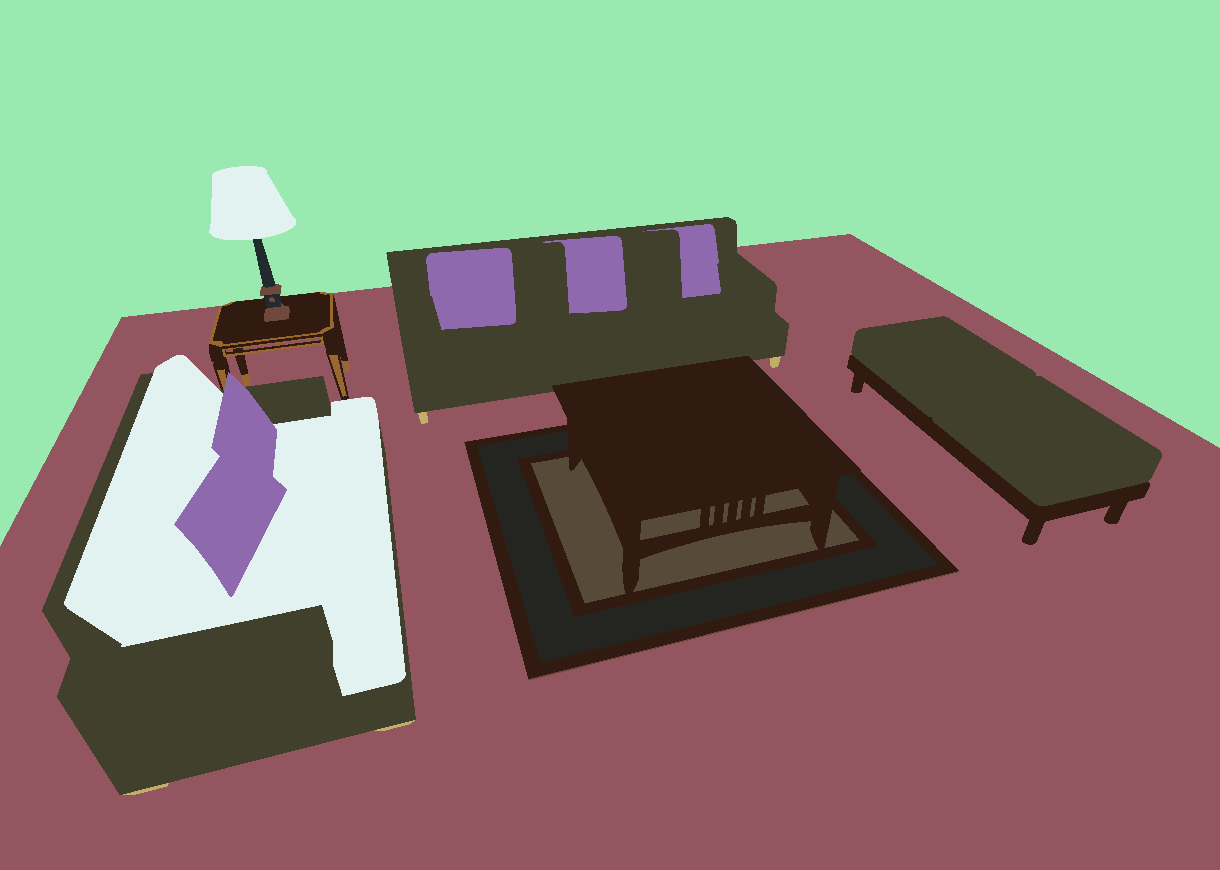
\includegraphics[width=.23\linewidth]{figs/3dscene/recolored_01}&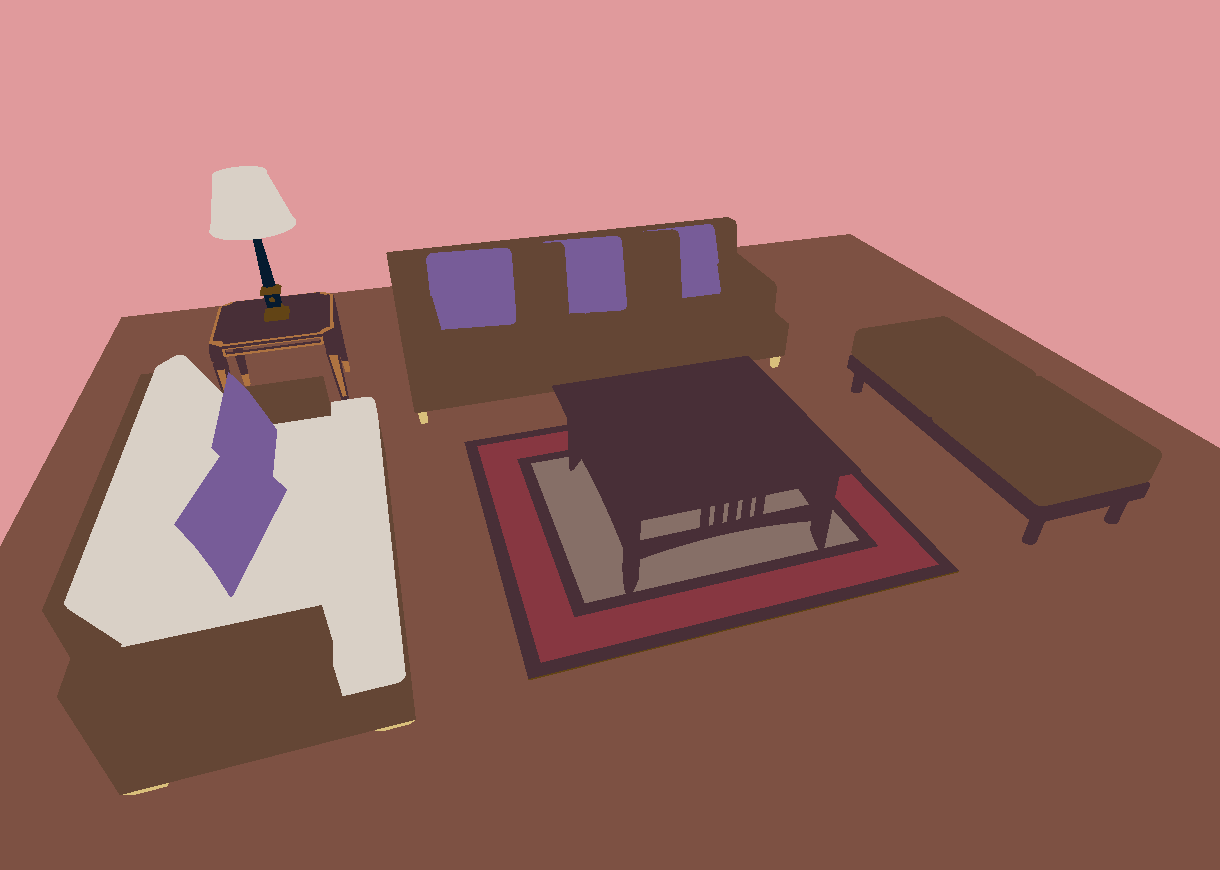
\includegraphics[width=.23\linewidth]{figs/3dscene/recolored_05}\vspace{0.4em}\\
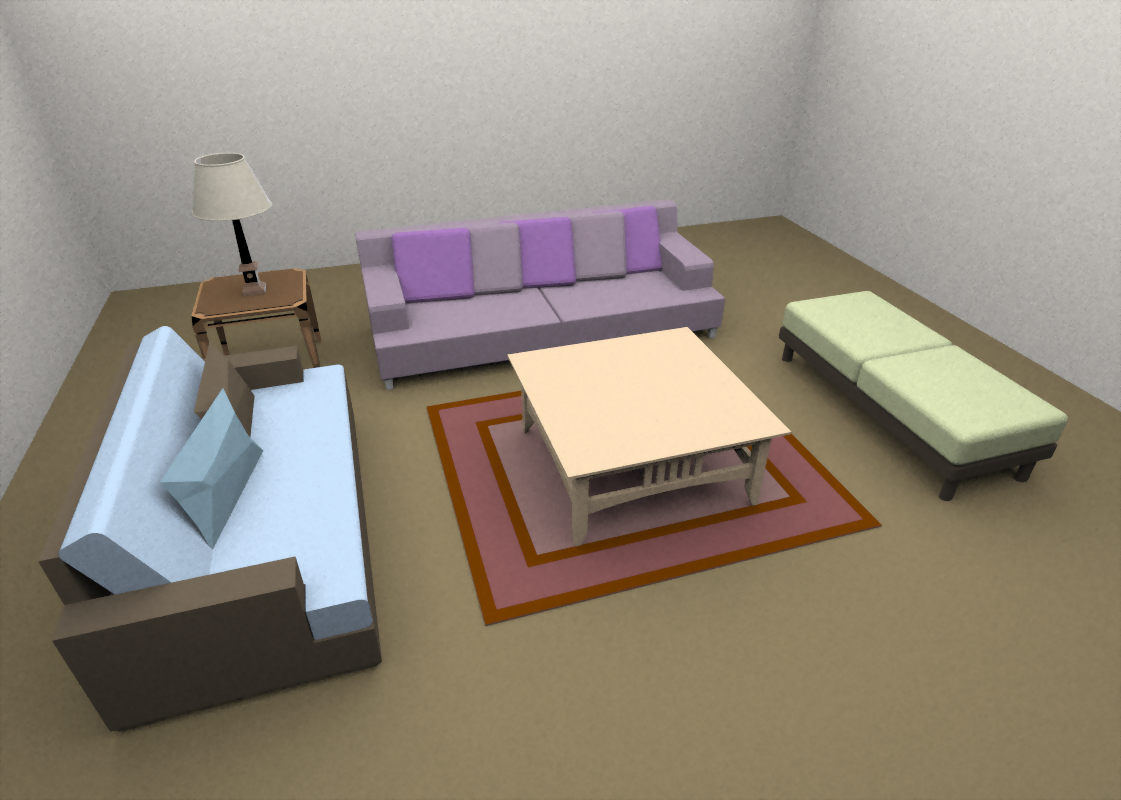
\includegraphics[width=.23\linewidth]{figs/3dscene/original_pbrt}&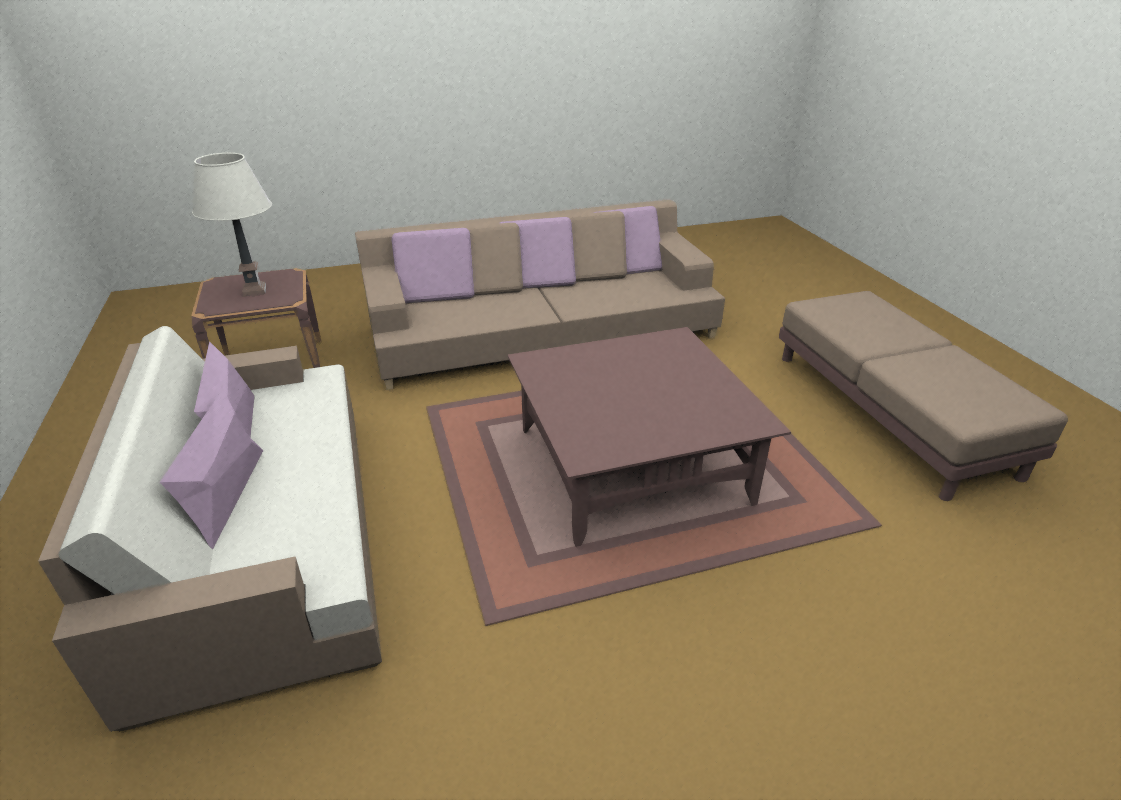
\includegraphics[width=.23\linewidth]{figs/3dscene/recolored_00_pbrt}&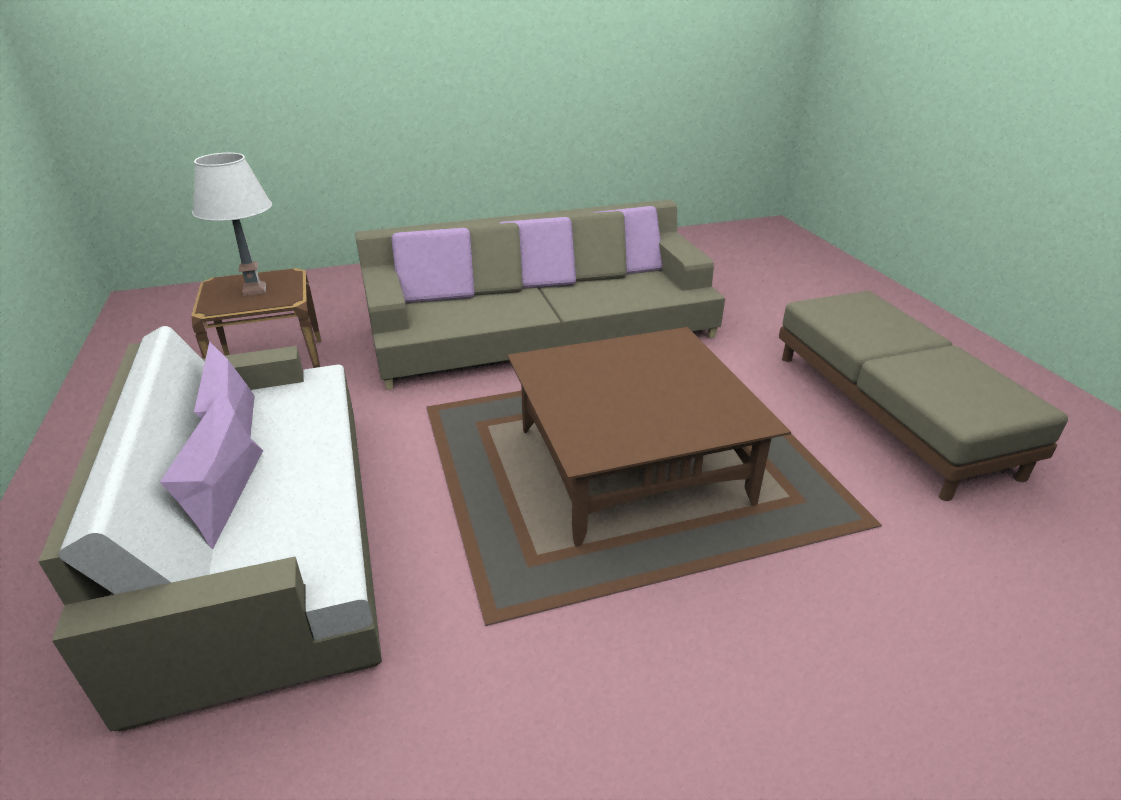
\includegraphics[width=.23\linewidth]{figs/3dscene/recolored_01_pbrt}&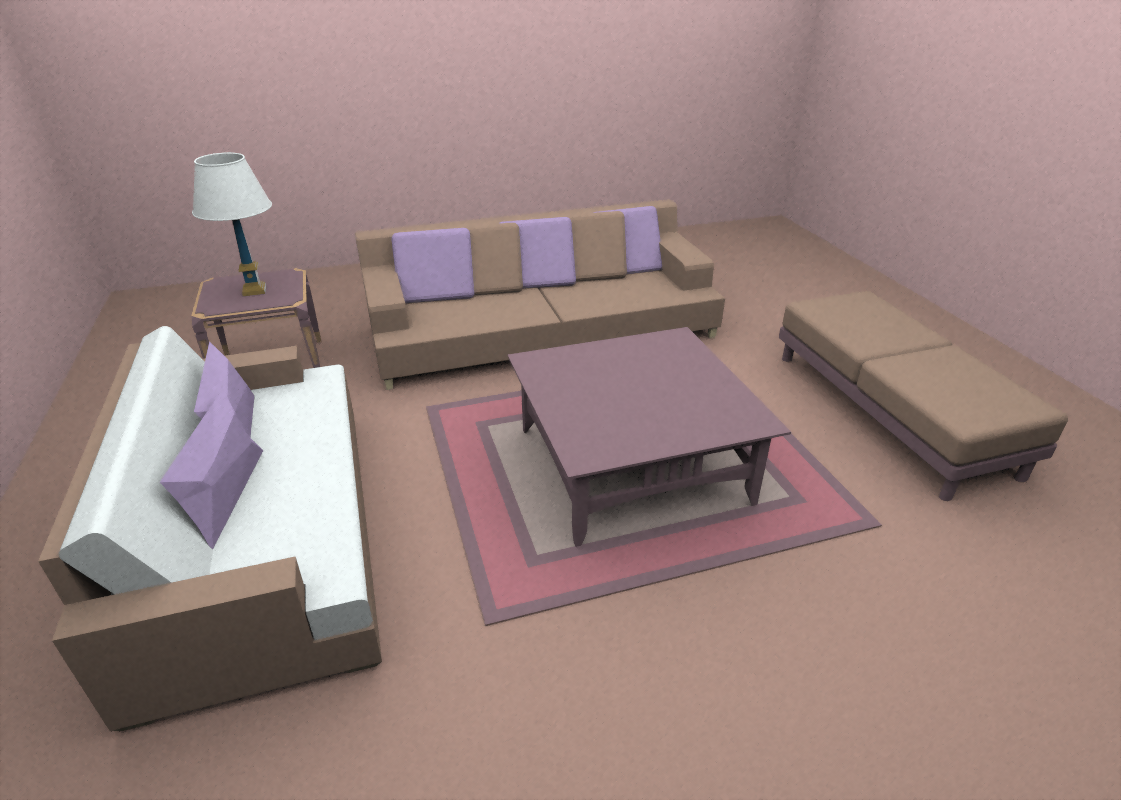
\includegraphics[width=.23\linewidth]{figs/3dscene/recolored_05_pbrt}\vspace{0.4em}\\
\end{tabular}

\caption{A poorly color-coordinated 3D scene is recolored using our model. Using the original coloring as a soft constraint, our model suggests multiple novel recolorings; here we show the top three suggestions. (Top) Diffuse material coefficients for each object. (Bottom) Final renderings of each scene.}
\label{fig:sceneRecoloring}
\vspace{-1.0em}
\end{figure*}

\paragraph{Fashion design}
Our model can also adapt the colorings of clothing items to fit different people. Figure~\ref{fig:fashion} shows a shirt recolored to match different hair, eye, and skin tones. The hair, skin, eyes, and lips of the 3D person model were manually quantized to a single color; the resulting texture atlas functions as a recolorable pattern template. Fixing the colors of the hair, skin, eyes, and lips constrains the inference process to produce suitable colorings for a person with those physical attributes. It should be possible to apply a similar procedure to photographic images, though those inputs may require an intrinsic image decomposition to separate shading from reflectance~\cite{IntrinsicImages}.

\begin{figure}[ht!]
\centering
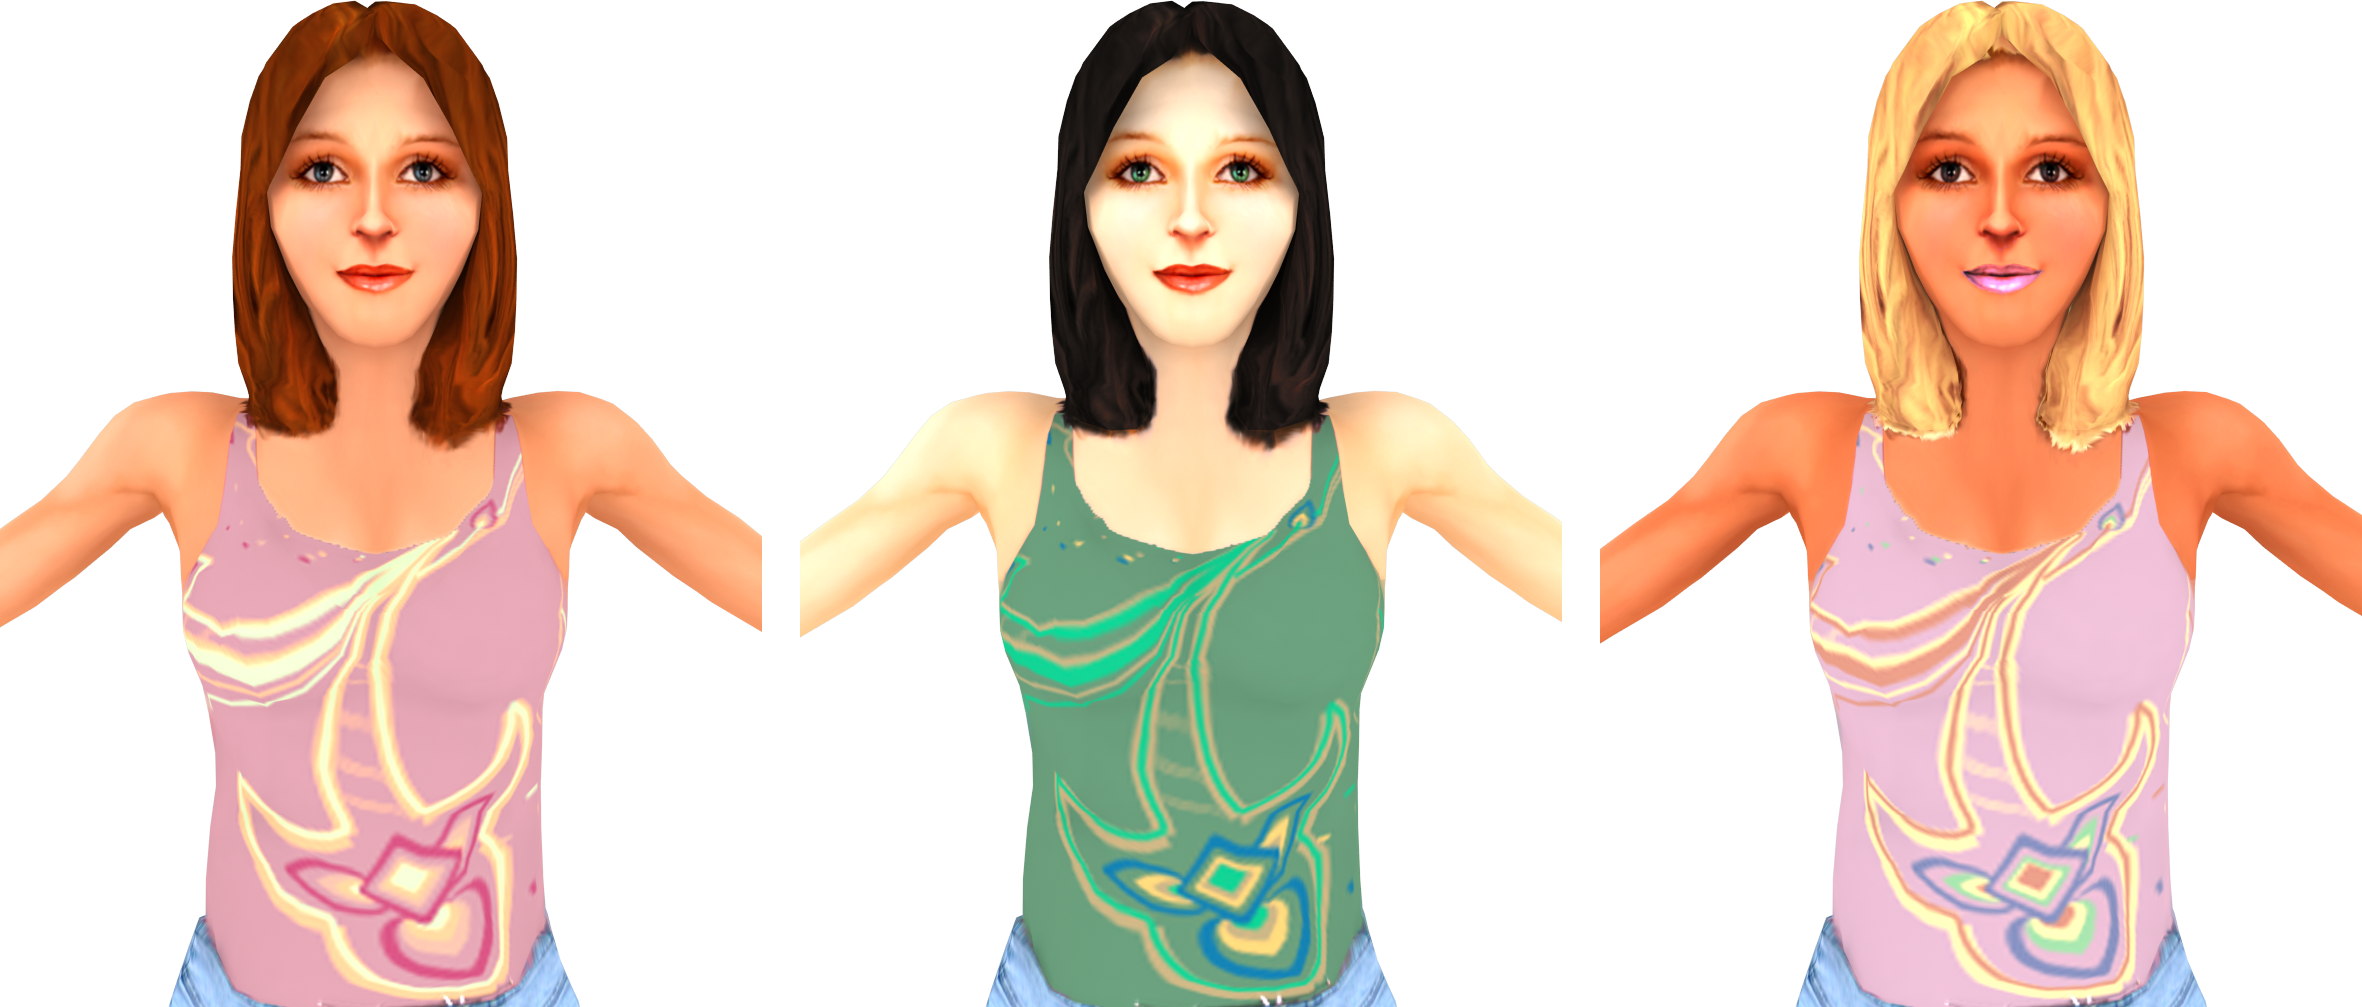
\includegraphics[width=\columnwidth]{figs/fashion/composite}
\caption{Using our model to colorize a patterned shirt for different people. The hair, skin, eye, and lip colors are treated as fixed constraints, which encourage the model to produce compatible colorings via adjacencies and long-range dependencies.}
\label{fig:fashion}
\end{figure}

\subsection{Performance}

The time required to generate coloring suggestions varies depending on the visual complexity of the pattern. Using the parallel tempering parameters described at the beginning of this section, the average sampling time was 73.0s to retrieve 20 MMR-diversified results for a single input pattern on a 2.67GHz Intel Core i7. Sampling is dominated by the probabilistic inference phase, which on average accounts for 83\% of the total running time.

Enabling real-time coloring suggestions would benefit many of the applications demonstrated in this paper, and there are several avenues for improving the performance of our unoptimized, JVM-based prototype to this end. We could leverage the massive parallelism of graphics hardware to speed up parallel tempering, as was done in related work on automatic furniture layout~\cite{MerrellFurnitureLayout}. We could also improve the convergence of the individual MCMC chains via gradient-based proposals, as in Hamiltonian MCMC~\cite{HamiltonianMCMC}. Prior work has shown the feasibility of computing the gradients of programmatically-expressed distributions using automatic differentation~\cite{AutoDiff}. 
\section{Evaluation}
\label{sec:evaluation}

%Results from MTurk experiment

% Motivation for evaluation design
% May be more general aspects of aesthetics that our model captures, compared to random colorings or color compatibility only
We conduct an evaluation on Mechanical Turk to gain a better idea of how coloring suggestions from our model compare to ones from simpler models as well as ones from artists. To better capture exploratory situations where our model would be used, we generate and present multiple coloring suggestions. Although different participants will have different aesthetic tastes, by looking across many participants, we should be able to see any general trends in the preferability of colorings generated by different methods. 

% Experiment Setup
We first generate a set of coloring suggestions from different sources -- artist colorings, our model, a color-compatibility-only model using the measure by O'Donovan et. al.~\shortcite{ODonovan}, and random colorings-- to be compared in the study. We picked 15 different pattern templates that do not have strong semantic associations and are also outside of our training set. Then, for each pattern template, we generated 4 coloring suggestions per source. For the artist source, we randomly picked 4 colorings from the top 45 artist colorings on COLOURlovers. For our model, we sampled colors using parallel tempering for 2000 iterations and picked the top 4 results using MMR with $\lambda = 0.5$. We similarly sample color-compatibility-only colorings. Finally, for the random source, we pick the first 4 random colorings.

The study interface presents participants with a randomized grid of suggestions for one pattern template at a time, for 6 pattern templates total. Participants are asked to pick the 4 colorings they think others will like the most and the 4 others will like the least from the grid for one pattern template before moving on to the next template. The order of pattern templates is randomized. In addition, one template is presented twice, to check for participant consistency. Each participant received \$X. We recruited a total of N participants for the study.

%\remark{We need acknowledge that yes, different Turkers will have different aesthetic sensibilities--but averaging across many of them, we should be able to see any general trends in the preferability of colorings generated by different methods.}

% Experiment Analysis
%We ran repeated-measures ANOVA on the number of suggestions picked as ``favorite 4'' and ``least favorite 4'' from each source. The suggestion source was set as a fixed effect and pattern templates and participants were set as random effects. [Results pending]

We use binomial regression to model the odds of each source being chosen--either as a top or bottom 4 suggestion. Tukey all-pair comparison tests show [Result pending]
\section{Discussion and Future Work}
\label{sec:discussion}

% Summarize, restate contributions.
In this paper, we present a probabilistic approach to automatically coloring 2D patterns. We develop a factor graph model that is trained on example pattern colorings to statistically capture their coloring style and sampled using MCMC to generate a variety of pattern coloring suggestions. We demonstrate the utility of the model on a range of coloring tasks, and a perceptual study showed that the colorings it generates compare favorably to those generated by other methods.

% Frame the discussion
There is still much work to be done to understand what makes a pattern coloring good. In this paper, we propose modeling one plausible set of color properties, and we gain some insight into which properties matter most by comparing their automatically-tuned weights. While colorings generated by the resulting model are attractive and useful, our evaluation shows that they do not yet achieve the same quality as colorings created by human artists. More research is needed to close this gap, and our probabilistic framework provides a strong and flexible foundation for further investigation.

% Discuss limitations, etc.
One immediate limitation of the current model is that it does not encode any semantic constraints on pattern regions, such as skies being blue or plants being green. This is not always a problem, as even human artists do not always respect these semantics (see the red clouds in Figure~\ref{fig:permutation}b), and patterns often admit many attractive, non-semantic colorings (Figure~\ref{fig:constrainedInference}). However, some patterns appear ugly or confusing when their colorings do not respect semantics, as shown in Figure~\ref{fig:badFlowers}. Labeling regions with semantic tags could address this problem, as the system could search for images on the web using these tags and build up a distribution of expected colors. It might even be possible to predict such labels automatically using sketch classification techniques~\cite{SketchClassification}.

In addition, some of COLOURlovers pattern templates use extensive color blending in their original vector artwork. For these patterns, the rasterized image is a poor approximation to the original artwork, and our model may not capture very predictive spatial features (or it may capture the wrong ones). In the future, we would like to apply our model to a dataset of vector patterns.

%~\remark{Other limitations/insights we may want to mention (at some point in the paper; it doesn't have to be here): (1) The fuzzy nature of probabilistic models means they may overshoot `hard' constraints that the viewer expects to be satisfied (e.g. some minimum contrast between adjacent regions). (2) For images that use blending extensively, the raster image is a poor approximation to the source vector artwork, and our model may not capture the features very well (or may capture the wrong ones). (3) Training simultaneously on many artists with different styles can yield `muted' results, as the model isn't confident about anything.}


\begin{figure}
\centering
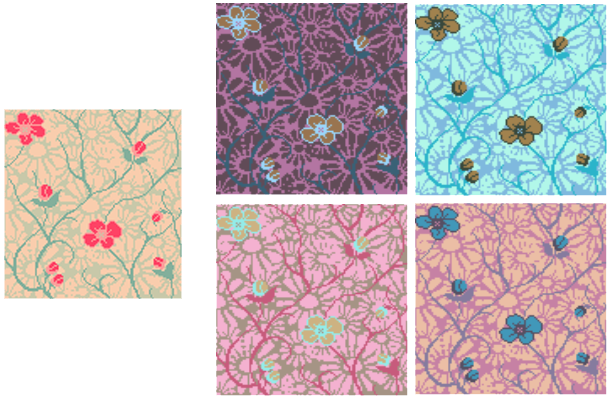
\includegraphics[width=0.7\columnwidth]{figs/badFlowers}
\caption{(Left) An artist's coloring of a pattern. (Right) High-scoring colorings of the same pattern sampled from our model. When the colorings do not respect the semantics of the flower stems by making them biologically impossible colors, it becomes difficult to parse the resulting image as one depicting a cluster of flowers.}
\label{fig:badFlowers}
\end{figure}


% Future work: Templatizing images
This research opens up several other interesting avenues for future work.
First, the results demonstrated in this paper use patterns from COLOURlovers or renderings that can be easily coerced into the same format. What if any image found `in the wild' could serve as a recolorable pattern template? As a simple first approach, we could extract a color theme from the image, and then quantize the image using the theme's colors~\cite{SharonPaletteExtraction}. Such a simple approach is unlikely to perform well on complex images that use many distinct colors, however. Solving the problem in general requires further research.

% Future work: Patterns where color groups are unknown
Second, this work explores colorizing patterns of the `color-by-numbers' format, in which some pattern regions are constrained to take the same color. What if this assumption were relaxed; that is, what if the color groups in the pattern template are unknown? A system that supported this more general type of pattern template could operate on an even larger set of inputs---essentially any image composed of segments. Implementing such a system would require a more sophisticated model, as well as transdimensional inference techniques to generate sample recolorings when the number of color groups is variable~\cite{YiTingLARJ}.

% Future work: Embed in real creative software
Finally, the prospect of embedding automatic coloring suggestions into real creative software presents an exciting opportunity. For example, a vector art program could continually generate suggestions in the background while its user works on a pattern; the user could choose to view the suggestions at any time, potentially picking one to use as an `autocompletion' of her work-in-progress. These kinds of tools have the potential to drastically shift the way that artists and enthusiasts work with color on a daily basis. 
%\section*{Acknowledgments}

Support for this research was provided by Intel (ISTC-VC) and an SAP Stanford Graduate Fellowship.
\remark{Other funding sources?}
We would also like to thank COLOURLovers \textit{jilbert} (Fig 1-4), \textit{symea} (Fig 1, 10), \textit{COLOURLover} (Fig 6, 12), \textit{timanttimaari}, \textit{dazzlement}, and \textit{ArrayOfLilly} (Fig 7), \textit{Any Palacios} (Fig 8-12), \textit{gregreis}, \textit{magg}, and \textit{praxicalidocious} (Fig 11), \textit{bhsav} (Fig 11, 12), \textit{vannea} and \textit{casslovescolors} (Fig 12), \textit{ivy21} (Fig 13), and \textit{caseycastille} (Fig 15) for their pattern templates; \textit{AlineDam} (Fig 9), and \textit{sugar!} and \textit{albenaj} (Fig 10) for the pattern coloring examples; and Flickr users \textit{marctasman} and \textit{zoomion} for the reference photographs (Fig 7).   


\bibliographystyle{acmsiggraph}
\bibliography{patternColoring}

\section*{Appendix}
\label{sec:appendix}

We provide more precise definitions for some of the color properties and features used in our model (Section ~\ref{sec:spatialCompat}).

\subsection*{Color Properties}

\begin{description}

\item[Unary] \hfill
	\begin{description}
	  \item[Colorfulness] measures saturation of a color in \lab space: $\frac{\sqrt{a^2+b^2}}{\sqrt{a^2+b^2+L^2}}$
	  %\item[Name Saliency and Name Counts] measure how uniquely a color is named and the distribution of names given to a color, as described in Heer and Stone ~\shortcite{ColorNamingModels}
	\end{description}
	
\item[Binary] \hfill
	\begin{description}
	  \item[Chroma Difference] measures the squared fraction of perceptual distance due to the chroma channels: $\frac{\delta a^2+\delta b^2}{\delta a^2+\delta b^2+\delta L^2}$
	\end{description}
	
\end{description}

\subsection*{Features}

\begin{description}

\item[Group Features] \hfill
	\begin{description}
	  \item[Relative Size] The total area of the group over the image area
	  \item[Segment Spread] 2D covariance matrix of the group's segment centroids
	  \item[Segment Size Statistics] the min, mean, max, and standard deviation of the group's relative segment sizes
	  \item[Number of Segments] The fraction of segments in the group out of the total number of segments in the image
	\end{description}
	
\item[Segment Features] \hfill
	\begin{description}
	  \item[Relative Size] The total area of the segment over the image area
	  \item[Normalized Discrete Compactness] measures compactness based on the relationship between the segment's boundary edges and its area ~\cite{NormalizedDiscreteCompactness}
	  \item[Elongation] measures the relative narrowness of a segment according to the width and height of its minimum area bounding box: $1-\frac{boxWidth}{boxHeight}$. A square is the least elongated.
	  \item[Label] A set of three binary values: {\emph{Noise}, \emph{Background}, \emph{Foreground}}. The \emph{Noise} variable indicates if the segment is a `noise' segment composed of small connected components. The \emph{Background} variable indicates if a segment belongs to the group with the largest connected component and is not `noise'. All other segments are labeled \emph{Foreground}.
	  \item[Radial Distance] measures Euclidean distance from the centroid to the center of the image
	\end{description}

\item[Adjacency Features] \hfill
	\begin{description}
	  \item[Enclosure Strengths] are two values which measure how much one neighbor in the adjacency encloses the other and vice versa. Enclosure strength is defined as the number of pixels of the neighboring segment appearing within a 2-pixel neighborhood outside the segment's boundary, normalized by the area of that neighborhood. Out-of-image pixels are counted as part of the neighborhood area.
	  \item[Unary Segment Features] The adjacency feature set also includes the segment feature vectors of the participating segments. We concatenate the two vectors, putting the one with the smallest $L_2$ norm first to enforce a consistent ordering.
	\end{description}
	
\end{description}

\end{document}
